% CT_Kylafi.tex
%
% Enjoy, evolve, and share!
%
% Compile it as follows:
%	xelatex demo.tex
%   bibtex demo.aux
%   bibtex lop.aux (run this, only if you pass option 'lop' below)
%   xelatex demo.tex && xelatex demo.tex
%
% Alternatively, compile it using `make -i' (see the provided Makefile).
%
% Check file `diphdthesis.cls' for other configuration options.
%
\documentclass[preface]{di_thesis}

%\usepackage{graphicx}

%%%%%%%%%%%%%%%%%%%%%%%%%%%%%%%%%%%%%%%%%%%%%%%%%%%%%%%%%%%%%%%%%%%%%%%%%%%%%%%
%%%%%%%%%%%%%%%%%%%% User-specific package inclusions %%%%%%%%%%%%%%%%%%%%%%%%%
%%%%%%%%%%%%%%%%%%%%%%%%%%%%%%%%%%%%%%%%%%%%%%%%%%%%%%%%%%%%%%%%%%%%%%%%%%%%%%%

\usepackage{booktabs}
\usepackage{hyperref}
\usepackage{amssymb}
\usepackage{amsmath}
% \usepackage{url,lineno,microtype,subcaption}
% \usepackage[onehalfspacing]{setspace}

% \usepackage{biblatex}
% \usepackage[backend=biber,
% style=alphabetic,
% sorting=ynt]{biblatex}
% \addbibresource{refs.bib}

\hypersetup{
    unicode=true,                     % non-Latin characters in bookmarks
    pdffitwindow=true,                % page fit to window when opened
    pdfnewwindow=true,                % links in new window
    pdfkeywords={},                   % list of keywords
    colorlinks=true,                  % false: boxed links; true: colored links
    linkcolor=black,                  % color of internal links
    citecolor=black,                  % color of links to bibliography
    filecolor=black,                  % color of file links
    urlcolor=black,                   % color of external links
    pdftitle={},                      % title
    pdfauthor={},                     % author
    pdfsubject={}                     % subject of the document
}
%%%%%%%%%%%%%%%%%%%%%%%%%%%%%%%%%%%%%%%%%%%%%%%%%%%%%%%%%%%%%%%%%%%%%%%%%%%%%%%
%%%%%%%%%%%%%%%%%%%% User-specific package inclusions %%%%%%%%%%%%%%%%%%%%%%%%%
%%%%%%%%%%%%%%%%%%%%%%%%%%%%%%%%%%%%%%%%%%%%%%%%%%%%%%%%%%%%%%%%%%%%%%%%%%%%%%%


%%%%%%%%%%%%%%%%%%%%%%%%%%%%%%%%%%%%%%%%%%%%%%%%%%%%%%%%%%%%%%%%%%%%%%%%%%%%%%%
%%%%%%%%%%%%%%%%%%%%%% User-specific configuration %%%%%%%%%%%%%%%%%%%%%%%%%%%%
%%%%%%%%%%%%%%%%%%%%%%%%%%%%%%%%%%%%%%%%%%%%%%%%%%%%%%%%%%%%%%%%%%%%%%%%%%%%%%%
%%%%%%%%%%%%%%%%%%%%%%%%%%%%%%%%%%%%%%%%%%%%%%%%%%%%%%%%%%%%%%%%%%%%%%%%%%%%%%%
%%%%%%%%%%%%%%%%%%%%%% User-specific configuration %%%%%%%%%%%%%%%%%%%%%%%%%%%%
%%%%%%%%%%%%%%%%%%%%%%%%%%%%%%%%%%%%%%%%%%%%%%%%%%%%%%%%%%%%%%%%%%%%%%%%%%%%%%%


%%%%%%%%%%%%%%%%%%%%%%%%%%%%%%%%%%%%%%%%%%%%%%%%%%%%%%%%%%%%%%%%%%%%%%%%%%%%%%%
%%%%%%%%%%%%%%%%%%%%%%%%%%% Required Metadata %%%%%%%%%%%%%%%%%%%%%%%%%%%%%%%%%
%%%%%%%%%%%%%%%%%%%%%%%%%%%%%%%%%%%%%%%%%%%%%%%%%%%%%%%%%%%%%%%%%%%%%%%%%%%%%%%
%
% First name, last name
%
% \authorFirstGr{Χριστίνα-Θεανώ}
% \authorFirstAbrGr{Χ.-Θ.} % abbreviation of first name
% \authorMiddleGr{Ε.}   % abbreviation of father's first name
% \authorLastGr{Κυλάφη}

% \authorFirstEn{Christina-Theano}
% \authorFirstAbrEn{C.-T.}
% \authorMiddleEn{E.}
% \authorLastEn{Kylafi}

% \authorAMSN{1115201200077}

%
% The title of the thesis
%
% \titleGr{Τίτλος πτυχιακής εργασίας στα Ελληνικά}
% \titleEn{BSc thesis title in English}

%
% Month followed by Year
%
% \dateGr{ΜΑΪΟΣ 2020}
% \dateEn{MAY 2020}

% %
% % Supervisor1 info
% %
% \advisorGr{Βασίλης Κατσούρος}
% \advisorRankGr{Ερευνητής Α'}
% \advisorOrgGr{Ε.Κ. "ΑΘΗΝΑ"}
% \advisorEn{Vasilis Katsouros}
% \advisorRankEn{Research Director}
% \advisorOrgEn{"ATHENA" R.C.}

% %
% % Supervisor2 info
% %
% \secadvisorGr{Ιωάννης Ιωαννίδης}
% \secadvisorRankGr{Καθηγητής}
% \secadvisorOrgGr{ΕΚΠΑ}
% \secadvisorEn{Yannis Ioannidis}
% \secadvisorRankEn{Professor}
% \secadvisorOrgEn{NKUA}

%
% The title of the thesis
%
\titleGr{Ανάπτυξη έξυπνου συστήματος συνοδείας τζαζ αυτοσχεδιασμού σε πραγματικό χρόνο}

%Εφαρμογή των Αναδρομικών Νευρωνικών Δικτύων για Αυτόματη Μουσική Συνοδεία σε Τζαζ Αυτοσχεδιασμό


\titleEn{iJazzARTIST: Intelligent Jazz Accompanist for Real-Time human-computer Interactive muSic improvisaTion}

%Adaptability of Recurrent Neural Networks in Real-Time Jazz Improvisation Accompaniment


%
% Month followed by Year
%
\dateGr{ΙΟΥΝΙΟΣ 2020}
\dateEn{JUNE 2020}

%
% First name, last name
%
\authorFirstGr{Χριστίνα-Θεανώ}
\authorFirstAbrGr{Χ.-Θ.} % abbreviation of first name
\authorMiddleGr{Ε.}   % abbreviation of father's first name
\authorLastGr{Κυλάφη}

\authorFirstEn{Christina-Theano}
\authorFirstAbrEn{C.-T.}
\authorMiddleEn{E.}
\authorLastEn{Kylafi}

% \authorAMSN{1115201200077}

%
% Supervisor1 info
%
\advisorGr{Βασίλης Κατσούρος}
\advisorRankGr{Ερευνητής Α'}
\advisorOrgGr{Ε.Κ. ``ΑΘΗΝΑ"}
\advisorEn{Vasilis Katsouros}
\advisorRankEn{Research Director}
\advisorOrgEn{``ATHENA" R.C.}

%
% Supervisor2 info
%
\secadvisorGr{Γιάννης Ιωαννίδης}
\secadvisorRankGr{Καθηγητής}
\secadvisorOrgGr{ΕΚΠΑ}
\secadvisorEn{Yannis Ioannidis}
\secadvisorRankEn{Professor}
\secadvisorOrgEn{NKUA}



%
% Members of the advisory board 
% (the first one, will be automatically taken up by the advisor)
%
% \boardTwoGr{Δεύτερο μέλος}
% \boardTwoRankGr{Βαθμίδα}
% \boardTwoOrgGr{Οργανισμός}
% \boardTwoEn{Second member}
% \boardTwoRankEn{Rank}
% \boardTwoOrgEn{Organization}


% \boardThreeGr{Τρίτο μέλος}
% \boardThreeRankGr{Βαθμίδα}
% \boardThreeOrgGr{Οργανισμός}
% \boardThreeEn{Third member}
% \boardThreeRankEn{Rank}
% \boardThreeOrgEn{Organization}

% %
% % 7 Member examination committee
% % (the first three will be taken up by the advisory board)
% %
% \examFourGr{Τέταρτο μέλος}
% \examFourRankGr{Βαθμίδα}
% \examFourOrgGr{Οργανισμός}
% \examFourEn{Fourth member} 
% \examFourRankEn{Rank}
% \examFourOrgEn{Organization}

% \examFiveGr{Πέμπτο μέλος}
% \examFiveRankGr{Βαθμίδα}
% \examFiveOrgGr{Οργανισμός}
% \examFiveEn{Fifth member} 
% \examFiveRankEn{Rank}
% \examFiveOrgEn{Organization}

% \examSixGr{Έκτο μέλος}
% \examSixRankGr{Βαθμίδα}
% \examSixOrgGr{Οργανισμός}
% \examSixEn{Sixth member} 
% \examSixRankEn{Rank}
% \examSixOrgEn{Organization}

% \examSevenGr{Έβδομο μέλος}
% \examSevenRankGr{Βαθμίδα}
% \examSevenOrgGr{Οργανισμός}
% \examSevenEn{Seventh member} 
% \examSevenRankEn{Rank}
% \examSevenOrgEn{Organization}

% %
% % The examination date of the thesis
% %
% \examinationDateGr{15 Μαΐου 2019}
% \examinationDateEn{May 15, 2010}
%
% Abstract, synopsis, inscription, ack, and preface pages.
%
% \abstractEn{This.}
% \abstractGr{Η περίληψη στα Ελληνικά.}
% \synopsisGr{Συνοπτική περιγραφή του διδακτορικού (5--8 σελίδες).}
% \acksEn{}
% \prefaceEn{}

\acksEn{










}
% \prefaceEn{

The thesis at hand is based on a collaborative project developed by the research team I had been part of, during my internship at ``Athena" Research Center. 

The research questions were initially formulated by Maximos Kaliakatsos-Papakostas, the project manager, and further developed by both Maximos and Kosmas Kritsis. The data processing, system design and implementation, as well as the experiments and results analysis, were a product of teamwork between Maximos, Kosmas and me. 

I would like to express my deep gratitude to my colleagues, Maximos and Kosmas for the wonderful cooperation and excellent guidance that I was given during the project and Maximos for his significant supervision of my thesis. I would also like to thank Vasilis Katsouros and Ioannis Ioannidis for their essential support during the overall process.



}


%\inscriptionEn{\emph{To my dear person.}}

%
% Subject area and keywords
%
% \subjectAreaEn{Subject Area}
% \subjectAreaGr{Θεματική Περιοχή}

% ------------------------------------------
\abstractEn{


Some of the most essential characteristics of improvisation on jazz standards are reflected through the accompaniment. Given a lead sheet as common ground, the study of the collaborative process of music improvisation between a human and an artificial agent in a real time setting, is a scenario of great interest in the MIR domain. So far, the approaches concerning the jazz improvisation accompaniment procedure, have presented systems that lack the capability of performing the accompaniment generation task while at the same time adapting to dynamically variable constraints depending on new, improvised data. The thesis at hand, proposes a jazz accompaniment system capable of providing proper chord voicings to the solo, while complying with both the soloist's intentions as well as the previously defined constraints set by the lead sheet. The artificial agent consists of two sub-systems; a model responsible for predicting the human soloist's intentions and a second system performing the task of the accompaniment. The latter is achieved by modeling the artificial agent's predictions, after exploiting the information on the expectations of the human agent's intentions, previously calculated by the first model. Recurrent Neural Networks (RNNs) comprise both aforementioned models. The dataset used in the training process has undergone multi-staged processing including probabilistic refinement, aiming to keep and enrich the information which is requisite for the task. The system was tested on two cases of jazz standards, demonstrating ability of compliance with the harmonic constraints. Additionally, output variability depending on the solo improvisation has been indicated. Emerging limitations as well as potential future perspectives are discussed in the conclusion of this work.


}
\abstractGr{

\begin{greek}

Κάποια από τα κυριότερα χαρακτηριστικά του αυτοσχεδιασμού σε πρότυπα τζαζ εκφράζονται μέσα από τη μουσική συνοδεία. Η συνεργασία μεταξύ ανθρώπων και τεχνητών συστημάτων για την επίτευξη αυτοσχεδιασμού σε πραγματικό χρόνο, υπό το πλαίσιο κοινής παρτιτούρας, αποτελεί ένα ιδιαίτερα ενδιαφέρον αντικείμενο μελέτης για τον τομέα της Ανάκτησης Μουσικής Πληροφορίας. Οι προϋπάρχουσες προσεγγίσεις που αφορούν στη διαδικασία της συνοδείας τζαζ αυτοσχεδιασμού, έχουν παρουσιάσει συστήματα που δε διαθέτουν την ικανότητα συμμόρφωσης με δυναμικά μεταβαλλόμενα περιβάλλοντα, εξαρτώμενα από τα αυτοσχέδια δεδομένα. Η παρούσα πτυχιακή εργασία παρουσιάζει ένα σύστημα συνοδείας, το οποίο διαθέτει την ικανότητα προσαρμογής τόσο στο τζαζ σόλο του μουσικού, όσο και τους περιορισμούς που έχουν προκαθοριστεί από την παρτιτούρα. Ο τεχνητός πράκτορας που αναπτύσσεται για το σκοπό αυτό, αποτελείται από δύο υποσυστήματα \textperiodcentered \ ένα μοντέλο υπεύθυνο για την παραγωγή προβλέψεων που αφορούν το σόλο του μουσικού κι ένα δεύτερο υποσύστημα που παράγει την τελική μουσική συνοδεία, αξιοποιώντας την πληροφορία για τις προθέσεις του σολίστα που παρήγαγε το πρώτο μοντέλο. Και τα δύο προαναφερθέντα μοντέλα έχουν ως σχεδιαστική βάση τα Αναδρομικά Νευρωνικά Δίκτυα. Το σύνολο των δεδομένων που χρησιμοποιήθηκαν στην εκπαίδευση των μοντέλων υποβλήθηκαν σε επεξεργασία πολλών επιπέδων, συμπεριλαμβανομένης της πιθανολογικής βελτιστοποίησης, με στόχο τη διατήρηση και την επαύξηση της χρήσιμης πληροφορίας. Το τελικό σύστημα εξετάστηκε με τη χρήση δύο τζαζ προτύπων, παρουσιάζοντας προσαρμοστική ικανότητα ως προς τους αρμονικούς περιορισμούς, καθώς και ποικιλομορφία, εξαρτώμενη από τον αυτοσχεδιασμό του μουσικού. Τέλος, αναφέρονται κάποιες δυσκολίες που προέκυψαν, όπως επίσης και προτάσεις για περαιτέρω έρευνα. 

\end{greek}

}
\subjectAreaEn{Machine Learning, Artificial Intelligence }
\subjectAreaGr{Μηχανική Μάθηση, Τεχνητή Νοημοσύνη }
\keywordsGr{αυτόματο σύστημα μουσικής συνοδείας, τζαζ αυτοσχεδιασμός, σύστημα \hspace*{3.4cm} μουσικής παραγωγής, βαθιά μάθηση, νευρωνικά δίκτυα μακράς βραχέας \hspace*{3.4cm} μνήμης, ανάκτηση μουσικής πληροφορίας, μηχανική μάθηση, αναδρομικά \hspace*{3.4cm} νευρωνικά δίκτυα, μουσικός αυτοσχεδιασμός
}

\keywordsEn{automatic accompaniment system, jazz improvisation, music generative \hspace*{2.7cm} system, deep learning, long short-term memory, LSTM, music information \hspace*{2.7cm} retrieval, machine learning, recurrent neural network, RNN, music impro- \hspace*{2.7cm} visation
}
%indentation
% \hspace*{2.6cm} 
\prefaceEn{

The thesis at hand is based on a collaborative project developed by the research team I had been part of, during my internship at ``Athena" Research Center. 

The research questions were initially formulated by Maximos Kaliakatsos-Papakostas, the project manager, and further developed by both Maximos and Kosmas Kritsis. The data processing, system design and implementation, as well as the experiments and results analysis, were a product of teamwork between Maximos, Kosmas and me. 

I would like to express my deep gratitude to my colleagues, Maximos and Kosmas for the wonderful cooperation and excellent guidance that I was given during the project and Maximos for his significant supervision of my thesis. I would also like to thank Vasilis Katsouros and Ioannis Ioannidis for their essential support during the overall process.



}

%
% Set the .bib file containing your paper publications (leave the extension out)
%
% This is optional, but it should be specified when option 'lop' is passed to
% the document class.
%
% Then, inside the document environment, you may use the command '\nocitelop' to
% site your papers, as you would traditionally do with the commands '\cite' or
% '\nocite'.
%
% The papers are printed in reverse chronological order.
%
%\lopfile{mypapers/pubs}
%%%%%%%%%%%%%%%%%%%%%%%%%%%%%%%%%%%%%%%%%%%%%%%%%%%%%%%%%%%%%%%%%%%%%%%%%%%%%%%
%%%%%%%%%%%%%%%%%%%%%%%%%%% Required Metadata %%%%%%%%%%%%%%%%%%%%%%%%%%%%%%%%%
%%%%%%%%%%%%%%%%%%%%%%%%%%%%%%%%%%%%%%%%%%%%%%%%%%%%%%%%%%%%%%%%%%%%%%%%%%%%%%%

% Center-justify "Contents", "List of Figures" , "List of Tables"
% Also, use Arial 14pt, bold font and capitalize
\renewcommand{\cfttoctitlefont}{\hspace*{\fill}\bfseries\fontsize{14}{1}\selectfont\MakeUppercase}
\renewcommand{\cftaftertoctitle}{\hspace*{\fill}}
\renewcommand{\cftlottitlefont}{\hspace*{\fill}\bfseries\fontsize{14}{1}\selectfont\MakeUppercase}
\renewcommand{\cftafterlottitle}{\hspace*{\fill}}
\renewcommand{\cftloftitlefont}{\hspace*{\fill}\bfseries\fontsize{14}{1}\selectfont\MakeUppercase}
\renewcommand{\cftafterloftitle}{\hspace*{\fill}}

% Indentation for toc entries
\cftsetindents{chapter}{0em}{2.5em}
\cftsetindents{section}{0em}{2.5em}
\cftsetindents{subsection}{2em}{2.5em}
\cftsetindents{subsubsection}{3.5em}{3em}

% fonts for toc entries (Arial 10pt)
\renewcommand\cftsecfont{\bfseries\fontsize{10}{1}\selectfont}
\renewcommand\cftsubsecfont{\fontsize{10}{1}\selectfont}
\renewcommand\cftsubsubsecfont{\fontsize{10}{1}\selectfont}

% Vertical space between toc entries
\renewcommand\cftchapafterpnum{\vskip8pt}
\renewcommand\cftsecafterpnum{\vskip10pt}
\renewcommand\cftsubsecafterpnum{\vskip8pt}
\renewcommand\cftsubsubsecafterpnum{\vskip8pt}


\begin{document}
\frontmatter

% site my papers
%\nocitelop{}

\mainmatter

% main chapters (should be given in capital letters)

\chapter{INTRODUCTION}
    %\section{MUSICAL COMPOSITION}
    Musical composition is about solving problems, while following certain instructions and rules. Musical styles are defined by constraints that need algorithmic solutions. As a result, each composition can be created by making a finite sequence of steps, as in every algorithmic process. Algorithms emerge, then, as the most appropriate tool for the creation and study of music. 
    
    %\section{MUSIC INFORMATION RETRIEVAL}
    A small but constantly growing field of research is the Music Information Retrieval (MIR) interdisciplinary science of retrieving music information. The applications of this field vary -- track separation and instrument recognition, automatic music transcription, automatic classification and music generation to name a few. MIR's aim is to extend the understanding and usefulness of music data, through research, development and application of computational approaches and tools. MIR is being used by businesses and academics to categorize, manipulate and even create music. %\subsection{FEATURE REPRESENTATION} 
    In order to perform data analysis, some summarisation of the information is required, which is achieved by the process of feature extraction. This is an important step, especially in cases that deal with audio content and application of machine learning techniques. The purpose of this task is to reduce the quantity of data down to a group of variables that are easily manageable in order for the learning procedure to be performed within a reasonable time period. Some examples of features in music data are diverse representations of the key, chords, harmonies, melody, main pitch, beats per minute or rhythm of the piece.

    %\section{MUSIC GENERATION}
    Over the past decades, there has been great interest in exploring AI methodologies for music generation. Several systems have been developed with manifold characteristics and nature. Having non-adaptive rule-based generative methods as a starting point and after years of advances in computational capacity, researchers have been employing more and more complex techniques to perform the task of music generation, such as probabilistic, deep-learning and evolutionary models. The tasks performed and matters researched vary, including collaborative human-computer music generation, jazz solo improvisation accompaniment and specific-style music generation. Deep Learning techniques in particular, have been widely used in recent research, due to the adaptive capabilities and pattern learning potential of such models, for instance, simple Recurrent Neural Networks (RNNs), Long Short-Term Memory Networks (LTSMs), Gated Recurrent Units (GRUs), attention based LSTMs and Bidirectional GRUs.


    \section{Motivation} \label{sec:motivation}
    Music conveys feelings and presents meaning on different levels of abstraction, while the mechanisms that stimulate emotions and make music interesting to humans are related to expectation and its fulfillment or violation \cite{huron2006sweet}, considering the engagement of the brain's predictive mechanisms in response to music \cite{margulis2007surprise}. Jazz improvisation is fundamentally based on the violation of expectation, conveyed through meaningful and novel improvised melodies, in live performances of jazz soloists or ensembles. Therefore, the task of jazz improvisation provides fertile ground for the study of the interaction between the anticipation and violation of expectation, the core-mechanism of music cognition.

    In order to create expressive jazz improvisations, effective communication between the collaborators is crucial, as well as certain role characteristics from each musician to be followed: 
    
    \begin{itemize}
        \item \textit{Expression of original ideas.} 
        
        Jazz musicians build up muscle memory through statistical learning from practicing and listening of musical pieces, an attribute that helps them combine or modify the jazz licks already learned in the process, so as to create their own music. The new, improvised phrases are considered to create meaningful violations of anticipation concerning the harmonic and rythmic characteristics, as discussed above.
        
        \item \textit{Interaction between the improviser and accompanist.} 

        During real-time jazz improvisations, the musical communication between the musicians is imperative. That is, in order to provide proper accompaniment to the improviser, the accompanist must continuously predict the intentions of the soloist and adapt to the solo improvisation.

        \item \textit{Adjustment to the harmonic and rythmic characteristics of the piece.} 

        While adapting to the soloist's improvisation style, the accompanist is considered to preserve the core attributes of the given jazz ``context", which stands as the common ground between the solo and the accompaniment. Commonly used alterations of the given melodies are new chords introductions, voicing additions and chord extensions, to name a few.
        
        
    \end{itemize}
    
    As a result of the above, a real-time system able to constitute an accompanist to jazz improvisations, is imperative to feature the following:
    
    \begin{itemize}
        \item[a.]   an anticipation model, related to the soloist's (human agent's) intentions.
        \item[b.]   adaptability to the playing style of the solo improviser.
        \item[c.]   ability of compliance to the harmonic and rythmic constraints of an input chart.
        \item[d.]   an enriched chord voicings vocabulary, able to provide diverse and creative accompaniment.
    \end{itemize}


        \subsection{Research Questions} \label{sec:researchQuestions}
        The thesis at hand, studies the characteristics of an artificial agent's accompaniment to a human jazz improviser in real-time, under a setting that simulates typical conditions of jazz improvisation, $e.g.$ defining previously agreed upon harmonic and metric constraints. Thus far, the approaches developed, generate static accompaniment to solos, compared to the methods discussed herein, proposing dynamic changes to the system's responses, which are dependable of the human solo improvisation. Deep Neural Networks have proven to be very efficient at capturing the statistical behaviour of large datasets, therefore the research purpose and questions of this thesis, focus on such models' suitability of being employed for the development of the system proposed in section \ref{sec:proposed_system} below.

        More specifically, this research, aims to answer the following questions:

        \begin{enumerate}
            \item[1.] Is the proposed system able to capture the static harmonic information of a given chart in a changeable setting? 
            \item[2.] To what degree does the deployed framework allow the system to respond to dynamic constraints dependable of the human agent?
            \item[3.] Is it feasible, in terms of computational complexity and robustness, to apply the presented setup in real-time performance?
        \end{enumerate}

        In this manner, the main contribution of this thesis is the study of a multi-layered NN, featuring integrated static and dynamic attributes, exploited to produce predictions for the accompaniment task described above.
        
        

    
    \section{Thesis Structure} 
    The rest of the thesis is organized as follows:

    \hyperref[chapter:related_work]{\textit{\textbf{Related Work}}} presents the state of the art in the research field of this thesis.

    \hyperref[chapter:theoretical_background]{\textit{\textbf{Theoretical Background}}} provides fundamental knowledge on concepts related to the scientific field of Machine Learning.

    \hyperref[chapter:materials_methods]{\textit{\textbf{Materials and Methods}}} includes detailed technical information about the implementation of the proposed system. 

    \hyperref[chapter:results]{\textit{\textbf{Results}}} presents the findings of the research procedure on the topic described in the \hyperref[sec:motivation]{\textbf{\textit{Motivation}}} section above.

    \hyperref[chapter:conclusions_futurework]{\textit{\textbf{Conclusions and Future Work}}} discuss further applications and research ideas aiming to improve the presented system.

\chapter{RELATED WORK} \label{chapter:related_work}
%Music generation is a broad subject and has been examined for %years, with researchers using multiple theoretical approaches and %methods for this task. 

    \section{Algorithmic Composition} 

    \subsection{Illiac} \label{subsec:illiac}
    Computer generated composition started with Lejaren Hiller and Leonard Isaacson at the University of Illinois in 1955, who used the Illiac high-speed digital computer to program basic material and stylistic parameters, which resulted in the Illiac Suite (1957). First, the score of the piece was composed and then it was transposed into musical notation in order to be read and performed by a string quartet. The process that Hiller and Isaacson have followed and resulted in the Illiac Suite, was to first generate certain ``raw materials" using the computer, then modify these materials according to multiple functions, and finally distinguish and select the best results from the modified musical materials according to various rules \cite{Alpern1995TechniquesFA}. 

    \subsection{MUSICOMP} \label{subsec:musicomp}
    The generator - modifier - selector paradigm explained in section \ref{subsec:illiac}, was also applied to MUSICOMP ( MUsic SImulator - Interpreter for COMpositional Procedures ), one of the first computer software developed for the purpose of simulating musical composition procedures, programmed by Lejaren Hiller and Robert Baker in Fortran and Scatre. Between the late 1950s and early 1960s, MUSICOMP composed the ``Computer Cantata". MUSICOMP was written as a library of subroutines, making the process of writing composition programs much easier, as the programmer-composer had the ability to use the routines within a larger program that suited his or her own style \cite{Alpern1995TechniquesFA}. The idea of building compact, well-defined compositional functions and then assembling them together, would prove efficient and provide the system a degree of flexibility and generality \cite{Alpern1995TechniquesFA}, which has made the aforementioned approach a popular one in many algorithmic composition systems, even to this day.


    
    \subsection{UPIC}
    UPIC (Unité Polyagogique Informatique CEMAMu) is a computerised musical composition tool, devised by the well-known composer Iannis Xenakis. UPIC's development was completed at the Centre d'Etudes de Mathématique et Automatique Musicales (CEMAMu) in Paris, 1977. Xenakis used it on his subsequent piece Mycènes Alpha (1978), and it has been used by several composers such as Julio Estrada, Jean-Claude Risset , François-Bernard Mâche, Takehito Shimazu, Mari King and Curtis Roads.

    Physically, the UPIC is a digitising tablet linked to a computer, which has a vector display. The user draws waveforms and volume envelopes on the tablet, which are showed on the computer. After the waveforms have been stored, the user can deploy them to create compositions, by drawing on the tablet, using the X-axis to represent time, and the Y-axis to represent pitch. The compositions can be stretched in duration from a few seconds to an hour. The compositions can be transposed, reversed, inverted and subjected to a number of algorithmic transformations. 

    \subsection{IBM 7090}
    Another pioneering application of the computer in algorithmic composition is that of Iannis Xenakis, who used the IBM 7090 computer's high-speed computations to perform calculations of various probability theories to aid in several compositions (such as Atrées (1962) and Morsima-Amorsima (1962) ). The program he created, would produce a score, making use of a list of note densities and probabilistic weights inserted by the programmer, specifying the duration and density of ``sound events", leaving the parameters of pitch, velocity, and dynamics to a random number generator. 


    \section{Non - Adaptive Generative Systems}
    
        \subsection{Stochastic Methods} \label{subsec:stochastic_methods}
        ``Stochastic" is a term from mathematics which designates such a process, ``in which a sequence of values is drawn from a corresponding sequence of jointly distributed random variables" (Webster's dictionary).
        
        ``Stochastic music" is based on a process in which the probabilities of proceeding from one state, or set of states, is [sic] defined \cite{audibleDesign}. The temporal evolution of the process is therefore governed by a kind of weighted randomness, which can be chosen to give everything from an entirely determined outcome to an entirely unpredictable one. In the stochastic method, a great number of the creative decisions concerning attributes and parameters, are merely left to chance.

        Such approaches, are characterised by randomness and can perform simple tasks such as generate a random series of notes, as in Mozart's Dice Music, while at the same time, a great amount of conceptual complexity can be introduced to the computations through the computer with statistical theory and Markov chains. Another example of non-computer-oriented ``stochastic" composition can be found in Karlheinz Stockhausen's Klaveirstucke XI. In this work, various music fragments are to be performed by a pianist in a random sequence. Additionally, Stochos \cite{Stochos} as described by the authors, is a real-time event generator implemented as a patch, allowing the assignment of stochastic, chaotic and deterministic curves to different sound transformation and synthesis parameters, through a control interface.

    
        \subsection{Rule - Based Approaches} \label{subsec:rule_based}

        A second approach to algorithmic composition using the computer is that of ``rule-based" systems and formal grammars. Musicologists have devised several abstract rules for defining musical style and for expressing what is ``allowed” in specific types of compositions \cite{maxim_kal_pap_book}. A rule-based process would center around those predefined rules, through which the program progresses. These steps are usually constructed in such a way that the product of the steps leads to the next new step \cite{burns1997algorithmic}. Rather than relying on randomness to make decisions as in the stochastic methods described in section \ref{subsec:stochastic_methods} above, rule-based systems pre-compose a ``grammar", by which the compositional process should behave, once set into motion.  This grammar, designates the formal system of principles by which the possible sentences of a language are generated \cite{burns1997algorithmic}, with, in this case, sentences being musical phrases. Like Hiller's MUSICOMP (\ref{subsec:musicomp}), the generative process usually takes the form of a computer program or a system comprising subroutines, often involving rules stored in databases, that were previously collected or newly invented. Examples of such approaches are the rule-based expert system for harmonization and Schenkerian analysis of chorales in the style of J.S. Bach, the CHORAL, presented by Kemal Ebcioğlu in 1988 \cite{choral_bach} and the approach of Phon-Amnuaisuk et al. \cite{phon2006chorale, Phon_bach_2002}, who introduced a Bach chorale style music knowledge representation, through expert-designed rules, enabling the user to control the developed system's harmonization behaviour.


        Non adaptive generative AI approaches, are based on proper mappings from processed data to musical surfaces for music generation. Cellular Automata, L-systems and non-adaptive/autonomous Swarm Intelligence, described in the following sub-sections are examples of such methods. The musical rules used by the aforementioned systems, are parts of this mapping, for instance, the output data of multiple generative algorithms is numerical, and each possible value produced is mapped to a musical object explicitly. This musical entity can be linked to pitch and/or rhythmic and/or intensity value and/or information related with structure. What renders the output musically meaningful is the design and development of that mapping. Additionally, coming up with proper mappings plays an important role in the system's creativity \cite{maxim_kal_pap_book}.


        \subsubsection{Cellular Automata} \label{subsub:ca}
        Cellular Automata (CA) are normally implemented on a computer as a regular array or matrix of variables, or cells, which normally can have one, two or three dimensions. Each cell may assume values from a finite set of integers and each value is normally associated with a colour. The functioning of such an automaton is monitored on the computer screen as a sequence of changing patterns of tiny coloured cells, according to the tick of an imaginary clock, like an animated film. At each tick of the clock, the values of all cells change simultaneously, according to a set of transition rules that takes into account the values of their neighbourhood \cite{miranda2001evolving}.   
        There have been several approaches at applying CA in the production of electronic music and sonic art, in the fields of overall structural composition, MIDI sequencing and sound synthesis/modification techniques to name a few. Reviews of such mappings can be found in Burraston and Edmonds \cite{burraston2005cellular}, Burraston and Martin \cite{burraston2006digital}, Miranda and Al Biles \cite{miranda2007evolutionary}. Other attempted approaches include symbolic music mapping from CA to notes (piece ``Horos'' by Iannis Xenakis \cite{solomos2005cellular}), similar mappings from CA to MIDI notes \cite{millen2004interactive}, audio synthesizing through granular synthesis, where the location of each active unit indicated which granule of sound would be active at any given time \cite{miranda2001evolving}, or from given spectrograms, where each unit was acting as an amplitude envelope for the respective frequency area of an input spectrogram \cite{serquera2010evolutionary}, as mentioned in Kaliakatsos-Papakostas \cite{maxim_kal_pap_book}.

        \subsubsection{Lindenmayer Systems}
        Lindenmayer Systems (L-Systems) were conceived as a mathematical theory of plant development by Lindenmayer in 1968 \cite{lindenmayer1968mathematical}. The original emphasis was on a mathematical model of cell development and plant topology, that is the neighborhood relations between cells or larger plant modules \cite{prusinkiewicz2012algorithmic}. The central concept of L-systems is that of rewriting, a technique for defining complex objects by successively replacing parts of a simple initial object using a set of rewriting rules. The typical and simplest form of L-systems belongs to the category of deterministic context free grammars(DOL-systems). As a form of formal presentation, the L-systems incorporate an alphabet $V$ of all possible symbols, a set of rules P that associates symbols in the alphabet with a string. Starting from an initial sequence of symbols $\ \omega \in V\textsuperscript{+2}$, denoted as $x\textsubscript{0}$, the rules are applied for each symbol in $x\textsubscript{0}$ resulting in a new sequence of symbols, denoted as $x\textsubscript{1}$. Recursively, the sequence $x\textsubscript{x+1}$ is formed by applying the rules in $P$ on each symbol in $x\textsubscript{n}$. After a number of k steps, the sequence $x\textsubscript{k}$ will constitute a symbol sequence that potentially exhibits interesting structural characteristics on many levels, i.e. not only neighbouring but also remote symbols. L-Systems, similarly to CA (section \ref{subsub:ca}), with their high-level structures are able to provide a sense of structural hierarchy when properly mapped to sound/music \cite{maxim_kal_pap_book}. Prusinkiewicz \cite{prusinkiewicz1986graphical} in his study, which was the first one to transform L-Systems to music, has directly interpreted the generated symbols to notes. McCormack \cite{mccormack1996grammar} has incorporated probabilities about rules associated with the symbols, creating mappings from symbols onto melodic notes. Other applications of L-Systems to music related research, cover sound generation \cite{manousakis2006musical}, the approach of Kaliakatsos-Papakostas et al. \cite{kaliakatsos2012intelligent}, where the produced strings at each next step were truncated to a fixed length, producing strings that had quasi-periodic characteristics at different level, proposing a variation of the L-systems, namely the Finite L-Systems (FL-systems), as well as the exploration of grammatical evolution of the musical FL-Systems' rules \cite{kaliakatsos2012genetic, maxim_kal_pap_book}.


        \subsubsection{Swarm Intelligence}

        Swarm Intelligence (SI) leads to the emergence of collective spatial behavior through the individual readjustment of the location of unique individuals, based on the application of simple rules that update the velocity of each agent according to the location and velocity of other neighboring agents \cite{maxim_kal_pap_book}. Reynolds \cite{reynolds1987flocks} introduced an algorithm in 1987, simulating swarm, herd and flock motion. This algorithm defines the motion of agent based on three components: shoaling, where each agent moves towards the center of mass of its neighboring agents, collision avoidance, where each agent moves away from the agents that are too close and schooling, where the velocity of each agent gets aligned with the mean velocity of the neighboring agents \cite{maxim_kal_pap_book}. Some of the aforementioned characteristics were incorporated to music and sound related interactive agents, developing multiple and wide-ranging approaches. SWARMUSIC \cite{blackwell2002improvised}, is an interactive music improviser, where a particle swarm algorithm generates musical material by a mapping of particle positions onto events in MIDI space, which was the first use of SI in a computer music application. Symbolic music composition has also been performed by such agents \cite{blackwell2003swarm}. Additive synthesis \cite{apergisSonoids2018}, granular synthesis \cite{blackwell2004swarm,blackwell2008swarm}  and granular synthesis with spatial characteristics \cite{wilson2008spatial}, are some more examples of SI applications. Finally, the sonification of the SI agents behavior has been integrated into the “Swarmlake” game \cite{kaliakatsos2014swarm}, which expanded the social behavior with user-controlled commands and attributed different agents with different sound properties, according to specific conditions of the game \cite{maxim_kal_pap_book}.


    \section{Adaptive Generative Systems}
    The multi-level nature of abstraction in musical works, makes even the most complex set of rules impotent to capture deeper patterns and structures, which necessitated the emergence of adaptive models in the field.
    Those kinds of models, have the ability to perform feature learning, explicitly or implicitly. After being trained on a dataset, they can capture the statistical behaviour of musical features either defined by the human agent(explicit methods) or extracted, abstract representations of them into feature latent spaces(implicit methods).

        \subsection{Explicit Learning}
        A music dataset may include explicitly defined features extracted from scores. Probabilistic generative models, are able to capture conditional and combined probabilities of such features; note occurrences, note transitions and conditional probabilities of chords over given notes, to name a few. After collecting statistical information about the dataset, multiple models can be trained, aiming at producing music that reflects characteristics of a given style. Examples of test cases are the four-part harmonisation (composition of a Soprano, Alto, Tenor and Bass (SATB) voice layout, combining those voices properly to form concise harmonic and melodic streams) \cite{allan2005harmonising,suzuki2013four} and the melodic harmonisation (composition of concise harmony over a given melody, without necessarily implementing compositions with specific voicing layout) \cite{simon2008mysong,raczynski2013melody}. Hidden Markov Models (HMMs) \cite{allan2005harmonising, simon2008mysong,raczynski2013melody} and more generalised Bayesian Networks (BNs) \cite{suzuki2013four} are able to perform tasks such as music modeling and generation, based on conditional probabilities across various elements of the dataset (\textit{e.g.} the probability of the current chord given the current observed note sequence).  \cite{maxim_kal_pap_book}. An interesting application of HMMs, MySong \cite{simon2008mysong}, produces chord sequences on the melody sung by the user, after extracting the melodic note fundamentals, with digital signal processing (DSP). The need to capture long-term structure was covered by deploying a recursive hierarchical generalization of the widely used hidden Markov models, the Hierarchical Hidden Markov Models (HHMM) \cite{thornton2009hierarchical}, which also preserve the generalisation capabilities of lower-order Markov models. In addition to the aforementioned approaches, graphical models able to capture long-term structure have also been proposed for modeling chord progression \cite{paiement2005probabilistic} as well as melodic harmonization \cite{paiement2006probabilistic}. Those models, use tree-like nodes that model conditional probabilities from top to bottom. 
        
              
        \subsection{Implicit Learning}
        
        \subsubsection{Machine Learning}
        Features can also be computed implicitly, without a transparent definition. Artificial Neural Networks (ANNs) as described further in section \ref{sec:nn}, are computational models, consisting of interconnected sets of artificial neurons. Typically, neurons are organized in recurrent networks with several interconnected layers. ANNs are used as a machine learning method and in the case of music, they process information from the musical surface and produce more abstract, non-transparent representations in each layer, with no distinction on which aspects of the musical surface are represented at each computational unit of the ANN. Implicit learning with deep ANNs offers important possibilities for categorization and prediction, without still giving clear information about what aspects of the data are more important for taking decisions. The recurrent or looped connections allow such networks to learn local dynamics of data and hold useful information across inputs resulting in developing a local memory. Recurrent neural networks (RNNs) are a class NNs that make use of sequential information in the dataset.
        Since music consists of sequences of musical elements(notes, chords, etc.), RNNs can be successfully employed in various musical applications as they store the data of the previously attended state. The most common are considered to be Long Short-Term Memory (LSTM) cells, described in detail in section \ref{subsec:lstm} and Gated Recurrent Units (GRU). Both of these architectures have multiplicative gates that protect their internal memory from being overwritten too easily, allowing them to handle longer sequences of data. To learn even longer-term structure, attention can be used. Attention is a later advancement, allowing models to access previous information without having to store it in the RNN cell’s state. In attention based LTSMs for example, certain components of the input at random moments can be ``attended" and utilized in order to produce portions of the network's output as opposed to simply output the final calculation of the last LSTM layer.
        

        \subsubsection{Approaches}
        The ANNs were first used during the 1970s and 1980s to analyze musical compositions, creating artificial models of cognitive theories of music \cite{todd1991music} but they were later adapted for music composition \cite{aiMethods}. Todd, who was the first to implement such networks in 1989, used a three-layered RNN that reproduces music in a specific style, but also allows the network to switch styles \cite{todd1989connectionist}. Given a set of one or more composition examples, the ANN was trained to associate a single input configuration to the output temporal sequence of the corresponding composition. Then, feeding input configurations different to the ones used during the training, created melodies interpolated between the ones used during the training. That means for example that if just one melody was used during the training, the result would be an extrapolation from it \cite{aiMethods}. Within the scope of melody generation, Mozer and Soukup examined the effect of psychoacoustical modeling of the inputs \cite{mozer1991connectionist} in 1991. In this method, the inputs and outputs were represented by a vector of coordinates related to pitch, the position(coordinates) on the chromatic circle as well as the position on the circle of fifths and the system was able to generate melodies in the style of Bach chorales \cite{maxim_kal_pap_book}. 

        To improve the aforementioned approach, Mozer proposed the first music generative system to use the recurrent networks technology (RNN's) in 1994, CONCERT (CONnectionist Composer of ERudite Tunes) \cite{mozer1994neural}, which was able to capture long-term structure of the learned melodies. CONCERT underwent training that involved a set of music data, from which the stylistic regularities were extracted, in order to compose new pieces. Significant improvements concerning long term structure was exhibited by deploying the Long Short-Term Memory ( LSTM ) networks, which are analysed in section \ref{subsec:lstm}) below. In Eck and Schmidhuber's approach \cite{eck2002learning}, the LSTM networks, include trainable gates that selectively forget information from the past or recall information from arbitrarily back in time, for generating blues melodies over a given blues chord progression. 

        Another approach for melody generation using LSTM RNNs was developed by Sturm et al. \cite{sturm2015folk}, where folk tunes (monophonic melodies) were modelled in the ABC format, a text and character-based representation that includes metadata, overview of musical setup ($e.g.$ tempo and time signature), metric information ($e.g.$ measure boundaries) and the music surface \cite{maxim_kal_pap_book}. Liang et al. presented a “quasi-monophonic” approach to modeling polyphonic data, where note symbols, bar limits and fermata(a symbol of musical notation indicating that the note should be prolonged beyond the normal duration its note value would indicate) symbols are learned and generated sequentially, from top to bottom and from left to right. In this approach, the ANN was fed with a sequence of single notes, where simultaneous notes simply had the same onset (beginning) time \cite{liang2017automatic}. 

        A similar representation approach with more refined information about the duration and offset time of notes was proposed by Colombo et al. \cite{colombo2018learning}, in which the ANN was fed with a sequence of single notes, where simultaneous notes simply had the same onset (beginning) time. Both of the aforementioned studies incorporated learning and generating polyphonic music in the style of Bach chorales, using LSTM units and Gated Recurrent Units ( GRUs ) respectively. In 2017, Hadjeres et al. introduced DeepBach \cite{hadjeres2017deepbach}, a graphical model based on RNNs, trained to generate four-part chorales in the style of J.S. Bach, which was made steerable by imposing constraints such as notes, rhythms or cadences in the generated score. Those constraints, allow the networks representing each voice(strand, melody or harmony of music within a larger ensemble or a polyphonic musical composition) to have a more robust understanding about the overall metric structure and the activity in each voice \cite{maxim_kal_pap_book}. The approach of Makris et al. for drums rhythm generation was similar to the approach of Hadjeres et al. \cite{hadjeres2017deepbach} in relation to constraints imposition. Indications were given that proper representation of the metric constraints could allow the network to compose rhythms in time signatures that were not encountered during training \cite{maxim_kal_pap_book}. 

        Chord progressions have been taken into account in more recent approaches. Choi et al. introduced text-based LSTM (Long Short-Term Memory) networks for automatic music composition in 2017, designed to learn relationships within text documents that represent chord progressions and drum tracks \cite{choi2016text}. Chu et al. presented a hierarchical multi-layer RNN, where the bottom layers generate the melody and the higher levels produce the drums and chords. Some researchers have also created hybrid systems, which means they combined ANNs with other methods. For example HARMONET \cite{hild1992harmonet}, is a model designed to solve the complex task of four-part choral harmonization in Bach’s style, an architecture comprising three-layers; a feed-forward ANN with a sophisticated encoding of musical information used to extract harmonization information, a rule-based constraint satisfaction algorithm for the chord generation and another ANN designed to add quaver ornaments to the previously generated chords \cite{aiMethods}. NETNEG \cite{lehmann1996netneg} was another hybrid system that combined NNs with rule based agents, an implementation aiming to create compositions of polyphonic music in real time. 
        
        Probabilistic methods can also be deployed in conjunction with ANNs. For example, the work of Verbeurgt et al. in 2004 , utilizes pattern recognition to extract patterns from musical training sequences, constructs a Markov chain the states of which are mapped to each pattern previously extracted and then deploys a neural network to learn which shifts of pitch and duration are allowed for each pattern in the training sequences \cite{verbeurgt2004hybrid}. 


    \subsection{Jazz Music Related Work}
    Jazz music has been in the centre of attention of many MIR research approaches. In 2017, Johnson et al. described a network trained to learn jazz melodies' musical structure over chord progressions, able to create improvised melodies, by calculating and assigning probabilities to prospective musical notes \cite{johnson2017learning}. Trieu and Keller presented JazzGAN in 2018, a generative adversarial network (GAN) using RNNs, for monophonic jazz improvisation over chord progressions, while at the same time introduced Mode Collapse, Creativity, and Chord Harmony metrics aiming for a better understanding and analysis of the musical quality of the generated sequences  \cite{trieu2018jazzgan}. The combination of music theory grammar with the LSTM architecture for jazz music generation, was another approach, presented by Wang et al. in 2019 \cite{wang2019jazz}. The input data of the LSTM model consists of interval, duration, and note category information extracted from MIDI files while the output of the model is a sequence of notes generated according to the transition probability, which is parsed according to the music grammar as the final step of the process. LSTM networks have been broadly used in research subjects involving jazz music composition, and more specifically music generation following the performer's style. 

    De Prisco et al. presented an approach consisting of a One-Class Support Vector Machine for learning the style of a jazz performer, a music splicing system for the composition of the melody following the previously learned style and a LSTM network to predict patterns constrained by the learned style and also guide the splicing system during the composition stage. Hori et al. \cite{hori2017jazz}, developed a complex automatic jazz accompaniment system, based on the stochastic state transition model which approximates a performance trajectory model. A LSTM network and a Deep Belief Network (class of deep neural network consisting of multiple layers, with connections between the layers but not between units within each layer) were also used,in order for the system to ``learn the correlation between the performance of the different jazz piano trio instruments from the performance MIDI data of jazz songs".
    
    
    \subsection{Real Time Applications}
    Real time scenarios however, are rare, with only a few approaches experimenting with or building such systems. Hidaka et al. introduced an automatic accompaniment system for jazz, able to capture the soloist’s intentions during the improvisation process and then output expressive accompaniment of a bass guitar and drums reacting to solo \cite{hidaka1995automatic}. Kaliakatsos-Papakostas et al. proposed a constraint-free improvisation environment, where the most important musical characteristics are automatically adapted to the human performer's playing style, without any prior information  \cite{kaliakatsos2012intelligent}. Differential Evolution (DE), Genetic Algorithms, FL-systems and statistical distribution modeling were employed in order to create the adaptive system, which provides automatic music accompaniment in real-time. Pachet has also proposed a system in 2010, the Continuator, which was able to learn and generate music in any style, either in standalone mode, as continuations of musician’s input, or as interactive improvisation back up in real time \cite{pachet2003continuator}. 



        %\subsection{MUSIC GENERATION}
        %\subsection{MELODY GENERATION}
        %\subsection{ACCOMPANIMENT GENERATION}
        %\subsection{INTERACTIVE GENERATIVE SYSTEMS}
        %\subsection{REAL-TIME ACCOMPANIMENT GENERATION}
    
    

\chapter{THEORETICAL BACKGROUND} \label{chapter:theoretical_backgroundpape}
    \section{Neural Networks (NNs)} \label{sec:nn}
    The human nervous system contains cells, called neurons. The neurons are connected to each another through axons and dendrites, the regions between which, are known as synapses(synaptic connections). In the presence of external stimuli, the strengths of synaptic connections are often differentiated, which is exactly how living organisms learn. 

      \begin{figure}[h]
        \centering
        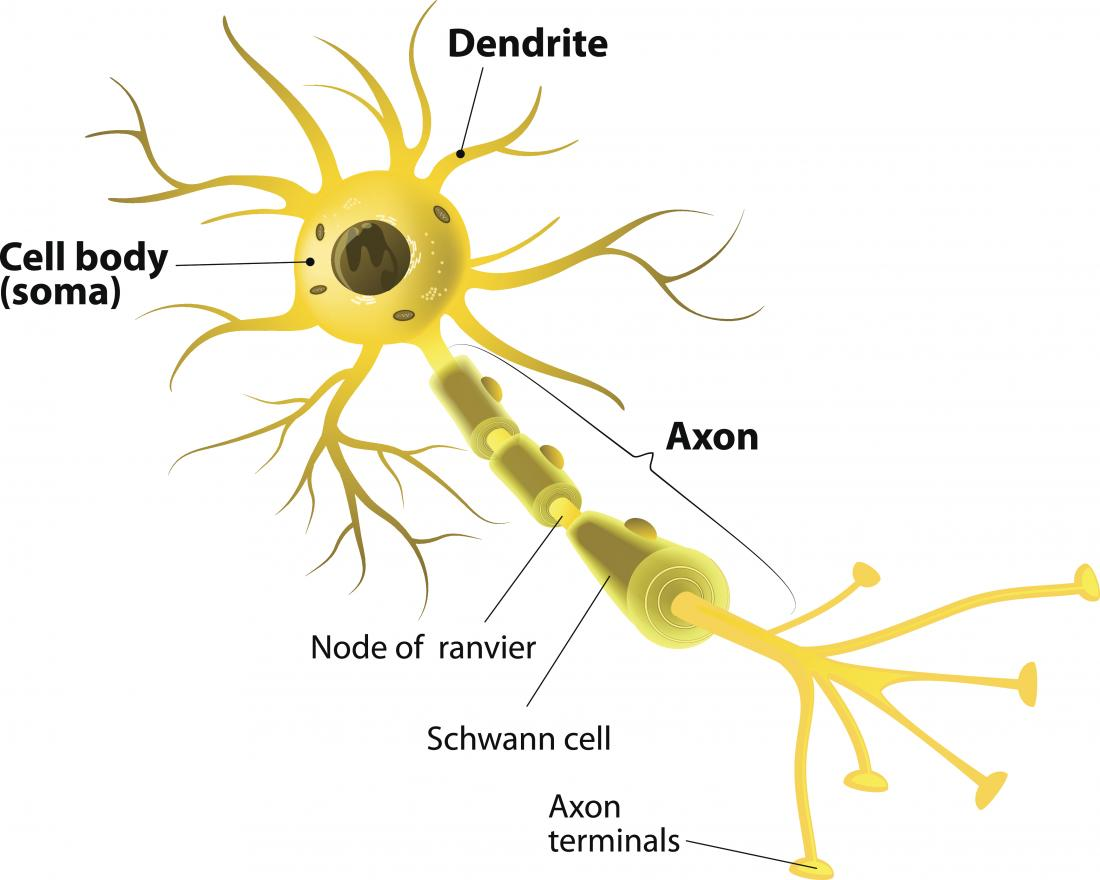
\includegraphics[width=0.65\textwidth]{media/neuron-diagram.jpg}
        \caption{Human Neuron}
        \label{fig:humanNeuron}
    \end{figure}

    
    Human neurons consist of three main parts: dendrites, the cell body and axons. Dendrites are thin filaments that carry information from other neurons to the soma of the neuron they are part of, so they are the input part of the cell. Soma (cell body) contains the neuron's nucleus and receives information through the dendrites. Axon is a long projection that transfers information from the soma to other cells in the system, so it is the output part of the cell. It normally ends with a number of synapses connected to the dendrites of other neurons.

    Artificial Neural Networks (ANNs) were made to mimic the biological mechanism explained above. They consist of units or nodes, referred to as neurons, which perform all the necessary computations. Those units are interconnected through weights, which have the same role as the strengths of synapses in the biological process. Each input to a neuron is scaled with a weight, which has impact on the function that this particular unit computes. An ANN computes a function of the inputs by propagating the computed values from the input nodes to the output node(s). The weights are parameters which undergo changes, in order for the learning process to take place. During that learning process, the network is being fed sets of training data containing examples of input-output pairs of the function to be learned, using the input representations to make predictions about the output labels. The training data provides the feedback needed to properly adjust the weights of the NN, a task that depends on how well the predicted output (e.g., probability of a C note -- Do) for a particular input, matches the output label in the training data. The goal of changing the weights is to optimise the computed function to predict more accurately in the next iterations. When a NN is trained with many different samples sharing the same label, it becomes capable of properly recognizing this label in input data not seen before. This ability of great accuracy in computing functions of unseen inputs by training over a finite set of input-output pairs, is called model generalization. This is exactly why machine learning models are gradually gaining ground in many fields, on the strength of their ability to generalize their learning from seen training data to unseen examples.
    
    \subsection{The Perceptron} \label{subsec:perceptron}
    The most simple NN, is called perceptron. It consists of only one input layer (collection of nodes operating together at the same depth within the NN) and an output node. Consider we feed the ΝΝ with training data, each instance of which is represented by pairs of the form (X,y), where X is a vector of k feature variables ( $X =  x\textsubscript{1}, x\textsubscript{2},...,x\textsubscript{k}$ ) and y is the observed value of the class variable for this specific set of feature variables ( $y \in \{class\textsubscript{1}, class\textsubscript{2},...,class\textsubscript{c}\}$ , where c is the number of total classes the NN is being trained to predict). The NN undergoes training in order to accurately predict the class variable, for unseen samples fed to the network as input. 
    The input layer, contains k units that connect the k feature nodes $X = [x\textsubscript{1}...x\textsubscript{k}]$ to an output node, through weighted edges, where $W = [w\textsubscript{1}...w\textsubscript{k}]$ are the weights of each edge with which the features are multiplied and added at the output node. 

    The input layer does not perform any computation. The linear function \begin{equation}
        W · X = \sum_{i=1}^{k} w\textsubscript{i} x\textsubscript{i} \label{eq:XY}
    \end{equation}
    which gives a real value that is used to predict the class variable depending on the input X, is computed at the output node. The selection of the function we use in order to map this real value to a class label, depends on the number and values of the classes. This function, is referred to as the activation function.
    For example, for binary classification( c = 2 classes ) where $y\in \{-1,\ +1\}$, it is preferable to use the sign function, which can give 2 possible results, -1 or +1, so the prediction y', is computed as follows: 
    \begin{equation}
        y' = sign\{ W · X\} = sign \{  \sum_{i=1}^{k} w\textsubscript{i} x\textsubscript{i} \} 
    \end{equation}  
    The error of the NN's prediction is 
    \begin{equation}
        E(X) = y - y', \quad where \ E(X) \in \{-2,\ 0,\ +2 \}.
    \end{equation}
    
    In case of a zero valued error, the prediction is accurate, so there is no change in the weights of the connections, whereas in case of a nonzero value, the weights are updated in the negative direction of the error gradient.
    In some cases, usually in imbalanced binary class distributions, part of the prediction is invariant and needs to be captured, e.g. in a setting with mean centered feature values, with non-zero mean, where $y \in \{ -1, +1 \}$ as before, an additional variable called bias is used: 
    \begin{equation}
        y' = sign\{ W · X + bias\} = sign \{  \sum_{i=1}^{k} w\textsubscript{i} x\textsubscript{i} + bias \}
    \end{equation}
    The bias can be incorporated as the weight of the edge connecting a neuron of a constant value of 1 to the output node.
    
   \begin{figure}[h]
        \centering
        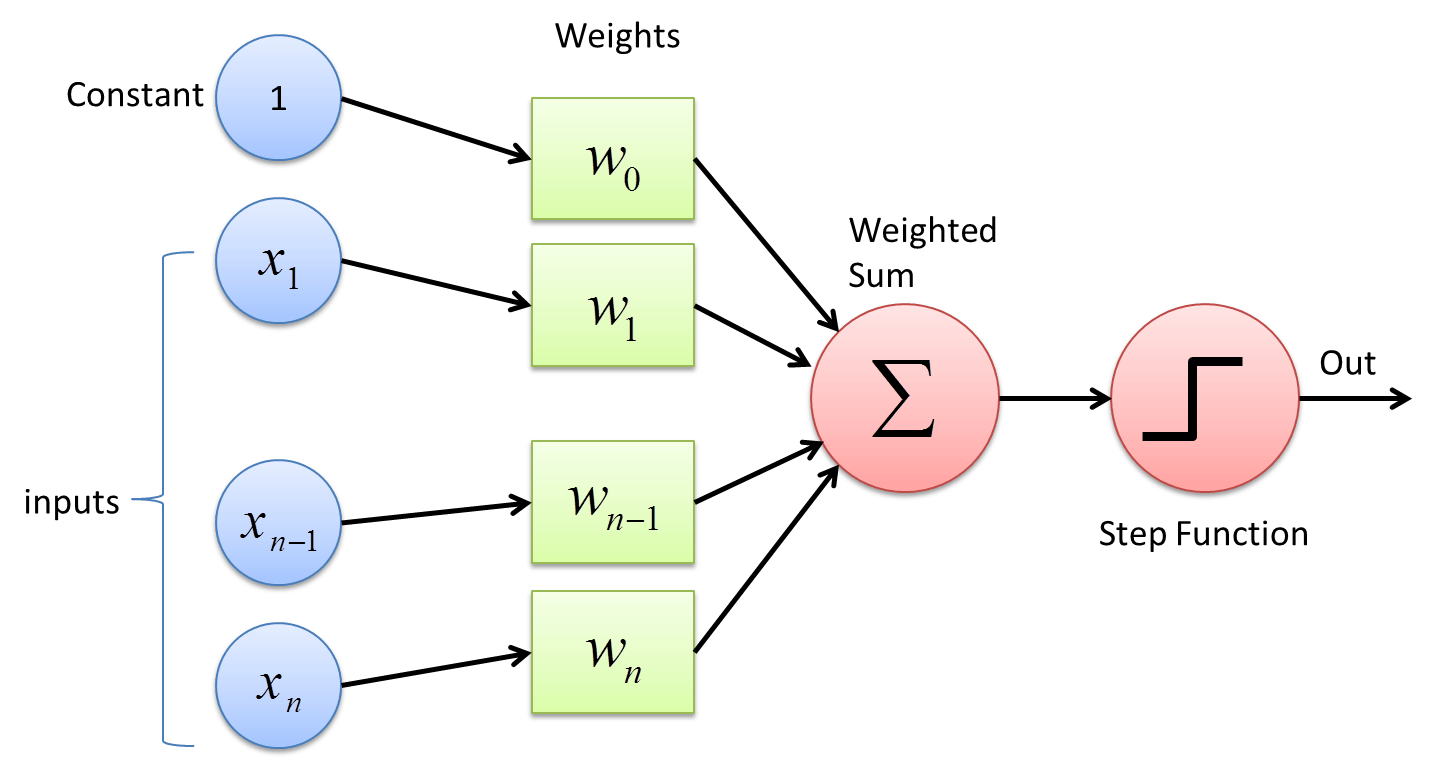
\includegraphics[width=0.50\textwidth]{media/perceptron.png}
        \caption{Perceptron model}
        \label{fig:perceptron}
    \end{figure}

    
    \subsection{Activation Function} \label{subsec:activation_funs}
    Τhe activation function defines the output of each node, given a set of inputs, that is, calculating the real value produced from \ref{eq:XY}.
    Multiple functions are used as activation functions in the development of NN's, such as the linear(identity), sign, sigmoid, hyperbolic tangent, ReLU, hard tanh and softmax functions. The fundamental activation function is the linear activation, which provides no non-linearity. Based on the type of classification combined with the number of classes, the most suitable activation is selected each time, so that the modeling power of the NN is the best possible for this task. The sign activation function, for example, can be used for binary classification. The sigmoid activation outputs a value y , where $y \subset (0,\ 1)$, which is preferable in cases of probabilistic computations(the prediction y' indicates the probability that the observed value, y, of the dependent variable is 1). The tanh function is usually used when the output of the computations is desired to be both positive and negative. Softmax results in probabilistic outputs, suitable for predicting one of multiple classes. ReLU is linear (identity function) for all positive values and zero for all negative values. The activation function is denoted by the symbol $\Phi$, so the prediction is calculated as follows: 
    \begin{equation} \label{eq:phi}
         y' = \Phi ( W · X  ) = \Phi ( \sum_{i=1}^{k} w\textsubscript{i} x\textsubscript{i} )
    \end{equation}
    where k is the number of input feature nodes. 
    Therefore, a neuron computes both functions of \ref{eq:phi} within the node.
   
    
    \subsection{Loss Function}
    Α loss(cost) function is a function that maps the value of one or more variables to a real number, representing the ``cost" of the event.
    The goal of the perceptron algorithm is to minimize the error in the prediction, therefore it is heuristically designed to minimise the number of misclassifications. The function that aims to minimise the value of the classification error(cost of classification), is called loss function. The choice of the loss function defines the outputs in a critical way and it is dependent on the application and the type of input data, as well as on the activation function used at that layer of the NN. In cases of numeric outputs, for example, a simple squared loss or hinge loss can be used. For a setting where the predictions are categorical, consider c the number of classes to be learned and y'\textsubscript{1},...,y'\textsubscript{c} the probabilities of the classes, with the rth class to be the ground-truth class, then for each instance, the loss function is calculated as follows: 
    \begin{equation}
        L = -\log(y'\textsubscript{r})
    \end{equation}
    This loss function is referred to as cross-entropy loss. 
    In detail, for each input data instance X or for a batch of them, the NN makes predictions used to calculate the error $E(X) = y - y'$, according to which the weights are updated. 
    The weight vector W is updated as follows:
    \begin{equation}
        W = W + a ( y - y' ) X
    \end{equation}
    The a factor controls the learning rate of the NN. What the perceptron algorithm does, is going over all the training data examples repeatedly in cycles and random order, while iteratively adjusting the weights until convergeance is achieved. Those cycles, are called epochs.
    
    \section{Feed - Forward Neural Networks}
    Multilayer NN's contain multiple hidden layers of computational units between the input and output layer. Those layers are referred to as hidden, because the computations performed are not visible to the user. Those successive layers, feed into one another in the forward direction from input to output. Those NN's, are known as feed-forward NN's. The number of nodes each layer has, is referred to as the dimensionality of this layer. In multi-layer networks, the loss is a complicated composition function of the weights in earlier layers.
    
    \begin{figure}[h]
        \centering
        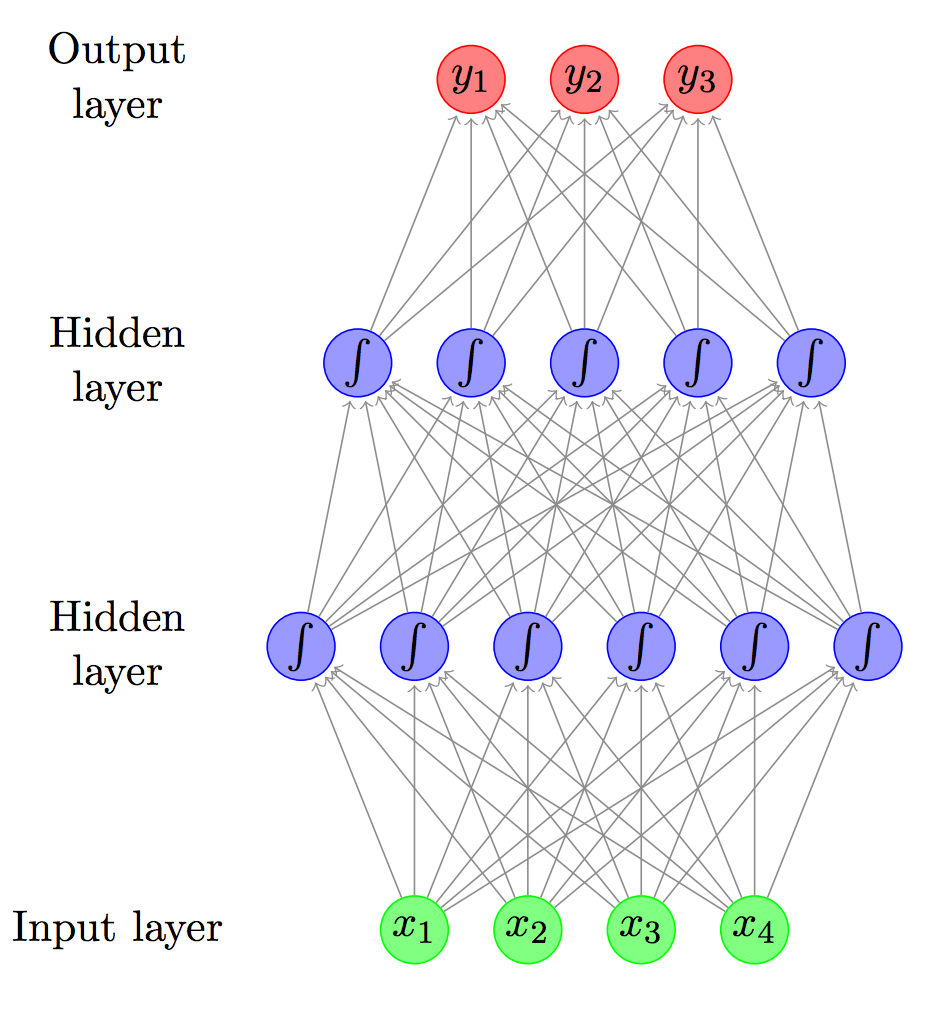
\includegraphics[width=0.50\textwidth]{media/Feed-forward-neural-network-with-two-hidden-layers.png}
        \caption{Feed-Forward NN structure}
        \label{fig:lstm}
    \end{figure}

    
    \subsection{Backprobagation}
    Multi-layer networks use various techniques in order to learn, the most popular of which is backpropagation. In this technique, the values produced by the NN as the output are compared with the correct answer, to calculate the value of the error function. The error is then fed back through the network, giving the information needed in order for the weights of each connection to be adjusted, so as to reduce the value of that error function as much as possible. After a large number of training cycles(epochs), the network will usually converge to a state where the computational error is small, which means that the NN was well trained and has learned a target function. 
    
    For the proper adjustment of the weights, a general method for non-linear optimization is used, referred to as the gradient descent. The network computes the derivative of the error function with respect to the network weights and changes the weights so that the error decreases (which means going downhill on the surface of the error function). That is the reason why backpropagation can only be applied on NN's with differentiable activation functions.

    The backpropagation algorithm contains two main phases, the forward and backward phase. During the forward phase the output and the loss are computed. Therefore, this phase initializes the intermediate variables that will be needed in the backward phase afterwards. The backward phase, uses the dynamic programming recurrence based on the multivariable chain rule of differential calculus. 
    More specifically, in the forward phase, the inputs for a training instance are fed into the NN, which results in a forward cascade of computations, where the values of each hidden layer are calculated, based on the current values of the weights across the layers. Those intermediate hidden and output variables will be required during the backward phase. After the completion of the computations, the prediction(final output) of the NN is calculated and compared to that of the training instance. Then, the derivative of the loss function with respect to the output is computed. The derivative of this loss afterwards, needs to be computed with respect to the weights in all layers in the backward phase.
    
    The main goal of the backward phase is to learn the gradient of the loss function with respect to the different weights by using the chain rule of differential calculus. These gradients are used to update the weights in all layers of the NN and are learned in the backward direction, starting from the output unit, where each node is processed exactly once in every pass. The learning process described above is known as the backward phase.
    
    \section{Recurrent Neural Networks (RNNs)} 
    
    \begin{figure}[h]
        \centering
        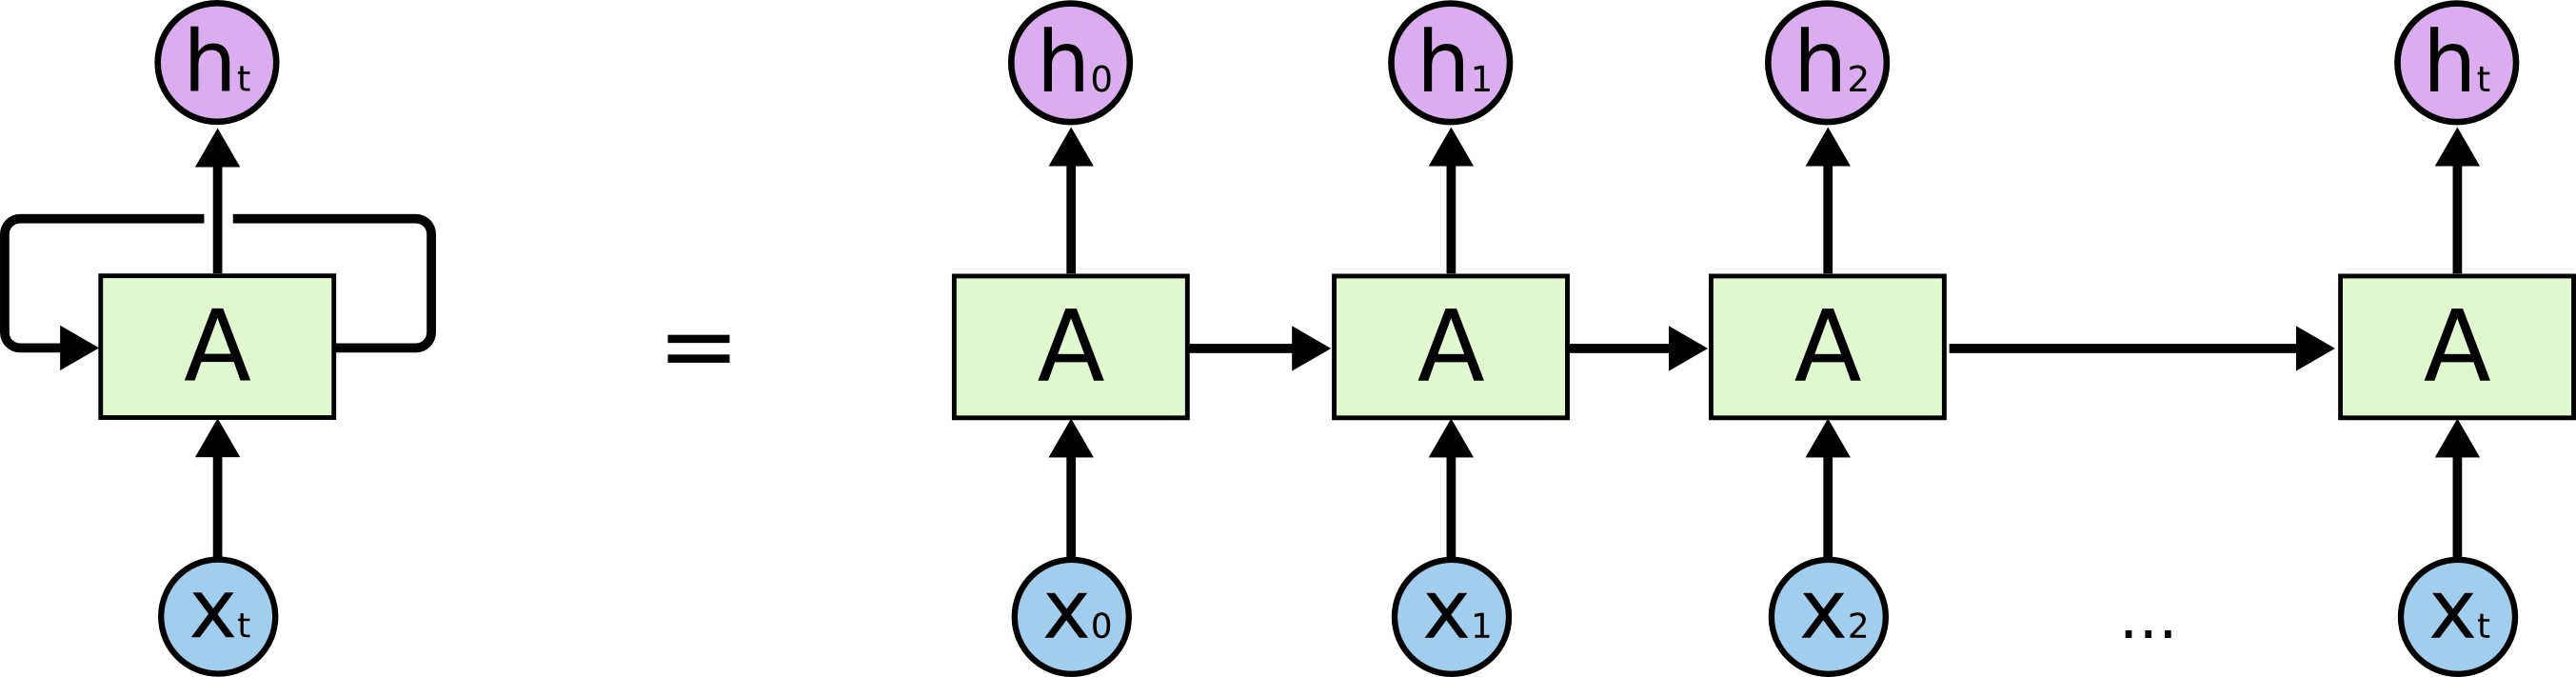
\includegraphics[width=0.65\textwidth]{media/RNN-unrolled.png}
        \caption{RNN unrolled}
        \label{fig:lstm}
    \end{figure}

    
    A recurrent neural network (RNN) is a feed-forward NN, where connections between nodes form a directed graph along a temporal sequence(series of items, e.g. a melody as a sequence of notes). This makes it capable of temporal dynamic behavior. This class of NNs can use their internal state (memory) to process sequences of inputs, unlike feed-forward NNs. The input of the RNN is an element x\textsubscript{t} of the sequence, where t represents the index or the time, and the expected output is next element x\textsubscript{t+1}. In other words, the RNN will be trained to predict the next element of a sequence. What makes the RNN capable to perform this task, is the action of reentering the hidden layer's output as an additional input. This way, the RNN can learn, not only based on the current item but also on its previous states, and thus, recursively, on the whole of the previous sequence. Therefore, an RNN can learn sequences, such as those of musical content. In such NNs, the input is of the form x\textsubscript{1} . . . x\textsubscript{n}, where x\textsubscript{t} is a d-dimensional point received at the time-stamp t. For instance, the vector x\textsubscript{t} might contain the d values at the t-th time-stamp of a multivariate time-series (with d different series). In a text-setting, the vector x\textsubscript{t} will contain the one-hot representation of the word at the t-th step . When a word is one-hot encoded, in a vector of length equal to the lexicon size, the component for this particular word has a value of 1 and all other components has a value of 0. The input x\textsubscript{t} of the RNN interacts with the hidden state produced from the inputs at previous time-steps, in a direct way. It is important that there is an input x\textsubscript{t} at each time-step, a hidden state h\textsubscript{t} that changes at each step as new data arrives and an output value y\textsubscript{t}. The hidden state at time-step t is given by a function of the input vector at step t and the hidden vector at step (t − 1): 
    \begin{equation}
        h\textsubscript{t} = f(h\textsubscript{t-1},x\textsubscript{t})
    \end{equation}
    The backpropagation algorithm in the case of RNNs, takes the temporal length into account when updating the weights during the learning process, which is a special type of algorithm, called backpropagation through time (BPTT).
    
    \subsection{ Long Short - Term Memory (LSTM)} \label{subsec:lstm}
    Training RNNs bears difficulties, due to the fact that they are deep time-layered networks, especially if the input sequence is very long. Thus, the depth of the temporal layering depends on the input data. However, even though the loss function has highly varying gradients to the variables in different layers, the parameter matrices are shared among different temporal layers, leading to unstable states. The main difficulties that emerge because of that, are the vanishing and exploding gradient during the update of the weights, specifically due to the successive multiplication of that shared weight matrix at backpropagation. A special class of RNNs, LSTMs, have been explicitly designed to deal with the vanishing gradient problem and they will be described below.
    LSTM is an RNN architecture which as such, has feedback connections and the ability to process not only single data points but also sequences of data, also capable of handling long-term dependencies. LSTMs have a chain like structure, where the repeating module consists of four NN layers, interacting in a very special way. The network's ability to model long-range dependencies and recognise patterns is achieved by using a gentle approach to update its cell states over time, so that there is greater persistence in the storage of certain information. Persistence in state values is exactly what eliminates the instability that occurs in the case of the vanishing and exploding gradient problems.

    \begin{figure}[h]
        \centering
        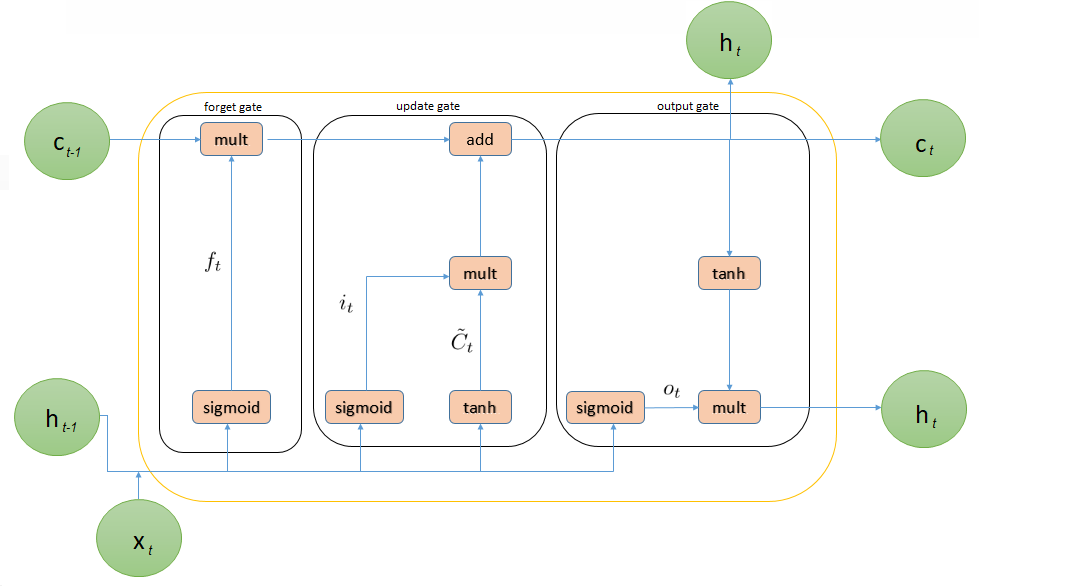
\includegraphics[width=0.65\textwidth]{media/lstm_simple.png}
        \caption{LSTM architecture}
        \label{fig:lstm}
    \end{figure}
    
    As we can see from figure \ref{fig:lstm}, there are three inputs (x\textsubscript{t}, h\textsubscript{t-1}, and c\textsubscript{t-1}) and two outputs (h\textsubscript{t} and c\textsubscript{t}) in the block, which are vectors carrying multiple values. Specifically, c\textsubscript{t-1} represents the input from a memory cell in time-stamp t, x\textsubscript{t} is a data input in step t, h\textsubscript{t} is the hidden state vector also known as output vector of the LSTM unit in time point t, that goes to both the output layer and the hidden layer in the next time-step. The key to LSTMs is the cell state, the line connecting input c\textsubscript{t-1} and output c\textsubscript{t} in figure \ref{fig:lstm} which runs straight down the entire chain of the NN, with only some minor linear interactions. It’s very easy for information to just flow along it unchanged. The LSTM has the ability to remove or add information to the cell state, controlled carefully by special structures, the gates. Gates optionally regulate the information that pass through. They consist of a sigmoid NN layer and a pointwise multiplication operation. The sigmoid layer produces numbers in range $( 0 \ 1 )$, a value that represents the percentage of each component to be let through. That is, based on the output of this sigmoid activation function, the valve will be completely closed, completely open or closed to some extent. A LSTM has three of these gates, to protect and control the cell state, which are called forget, update and output gates. For instance, when the forget valve(gate) in figure \ref{fig:lstm} above is open, memory flows from c\textsubscript{t-1} to c\textsubscript{t}. On the other hand, when the valve is closed, memory is cut off, and probably new memory will be added further in the pipeline.

    Specifically, the gates perform the following tasks:
    \begin{itemize}
        \item 
        The forget gate, manages what portion of the information from the previous state will be kept in the next state. It takes in the previous cell output h\textsubscript{t−1} and the current input band x\textsubscript{t}, applies the sigmoid activation layer so as to get values $\in (0,1)$, for each number in the cell state c\textsubscript{t−1} (equation \ref{eq:f}) and then performs element-wise multiplication with the old state from the previous unit.

        \item
        The update gate, updates the cell state based on the current input, by passing h\textsubscript{t−1} and x\textsubscript{t} into both a sigmoid activation layer (\ref{eq:i}) and tanh activation layer (\ref{eq:cellUpdate}), performing then an element-wise multiplication between the two results. The result from the previous operation is element-wisely added to the current state after applying the forget gate, to update the state with new information (equation \ref{eq:cellState}).    
       
        \item 
        Finally, the output gate controls what information gets passed on to the next state. A tanh activation layer is applied on the current state, to push the values in range $(-1,\ 1)$ and then an element-wise multiplication is performed, with the cell input (h\textsubscript{t−1} and x\textsubscript{t}) run through a sigmoid layer acting as a filter on what we decide to output. The output h\textsubscript{t} is then passed to the next layer of our network as one of the inputs.
        
    \end{itemize} 
    
    Therefore, summing up all of the above and as we can see from figure \ref{fig:lstm}, an LSTM unit takes x\textsubscript{t}, h\textsubscript{t-1}, and c\textsubscript{t-1} as inputs and after all the calculations and applications of its layers, it produces the h\textsubscript{t} and c\textsubscript{t} as outputs, which will be the inputs of the next LSTM unit, along with the data input of the next time-step  x\textsubscript{t+1}. The input x\textsubscript{t} is d-dimensional and the hidden states of the network are p-dimensional. The updates use four intermediate, p-dimensional vector variables $i,\ f,\ o$ and $C$. The intermediate variables $i,\ f$ and $o$ are respectively called input, forget, and output variables, because of the tasks they perform in the process of updating the cell and hidden states. Matrices $W \in \mathbb{R}\textsuperscript{$p\ x\ d$}$ and $U \in \mathbb{R}\textsuperscript{$p\ x\ p$}$ are the weight matrices and $b \in \mathbb{R}\textsuperscript{$p$} $ is the bias vector parameters, which all need to be learned during training, where $p$ is the number of hidden units and $d$ the number of features of the input data, as mentioned above.
    
    First, $f\textsubscript{t}$, $ i\textsubscript{t}$ and $ \Tilde{C}\textsubscript{t}$  are computed as follows:
    \begin{equation} \label{eq:f}
        f\textsubscript{t} = \sigma(\ W\textsubscript{f}\ x\textsubscript{t} + U\textsubscript{f}\ h\textsubscript{t-1} +  b\textsubscript{f}\ )
    \end{equation}
    
    \begin{equation} \label{eq:i}
        i\textsubscript{t} = \sigma(\ W\textsubscript{i}\ x\textsubscript{t} + U\textsubscript{i}\ h\textsubscript{t-1} +  b\textsubscript{i}\ )
    \end{equation}

    \begin{equation} \label{eq:cellUpdate}
        \Tilde{C}\textsubscript{t} = tanh(\ W\textsubscript{C}\ x\textsubscript{t} + U\textsubscript{C}\ h\textsubscript{t-1} +  b\textsubscript{C}\ )
    \end{equation}

    Then, the old cell state needs to be updated as well:
    
    \begin{equation} \label{eq:cellState}
        C\textsubscript{t} = f\textsubscript{t} * C\textsubscript{t-1} + i\textsubscript{t} * \Tilde{C}\textsubscript{t}
    \end{equation}

    Finally, the output will be computed, based on a filtered version of the updated cell state above, as follows:

     \begin{equation}
        o\textsubscript{t} = \sigma(\ W\textsubscript{o}\ x\textsubscript{t} + U\textsubscript{o}\ xh\textsubscript{t-1} +  b\textsubscript{o}\ )
    \end{equation}
    
    \begin{equation}
        h\textsubscript{t} = o\textsubscript{t} * tanh\ (C\textsubscript{t})
    \end{equation}
    
    


\chapter{MATERIALS AND METHODS} \label{chapter:materials_methods}
    \section{Proposed System} \label{sec:proposed_system}
    The general idea was to create a system that would be able to provide accompaniment to a human soloist, based on given lead sheet chords, in real time. The system's task is to interpret the information given from the lead sheet with variability, depending on the predicted harmonic variability of the human solo. In order for the system to do so, data need to include information about the following:
    
    \begin{itemize}
        \item Metric structure
        \item Human solo channel
        \item Accompaniment channel
        \item Lead sheet information
    \end{itemize}
    
    Providing the system with all the information above, it will have the ability to recognise measure changes, respond to the expected human solo and learn to comply with the given lead sheet chords, resulting in producing proper accompaniment for the human solo.

    \section{Data Preprocessing}
    Due to the lack of a readily available dataset that includes all of the information above, a need of such emerged. This section describes the exact procedures that were followed, $e.g.$ modification and augmentation of the original dataset, to create a proper dataset for the task of the system training.

        \subsection{Description of the dataset} \label{subsec:initial_dataset}
        The initial dataset\footnote{\url{https://github.com/wayne391/lead-sheet-dataset/} -- last accessed October 27 2019.} \cite{liu2018lead}, carries information about the pieces that are included -- the tempo, beat, melody and chords on the lead sheet. The beat information indicates the measure structure. One time-stamp corresponds to 1/24 of a quarter note, a time resolution able to represent rhythm values of even sixty-fourth triples. The melody and the accompanying chords are saved as 128-keys piano roll representations with the time resolution mentioned above, where the note that is played at each time-step, is indicated by its velocity value. However, following this type of representation, a possible note repetition cannot be clear, as there is not a way to distinguish one single quarter (note or chord) held for 24 time steps, from two successive eighths (notes or chords) each one held for 12 time steps. 

        \subsection{Time Resolution} \label{subsec:time_resolution}
        The time resolution was reduced, from 24 time-steps per beat(quarter) to 2 steps per beat, in order for each time-stamp to represent an eighth note, which is half the duration of the quarter. To perform this task, from each beat that lasts 24 time-steps, only the information that is indicated by the first and the thirteenth step is kept. More specifically, the followed procedure involves splitting each quarter in half, in order to create two subsets of 12 time-steps each and then keeping only the first step of each subset. As a result, the initial quarter was replaced by two eighths, with a new resolution of 2 instead of 24 time-steps each.
        
        \subsection{Chord Information} \label{subsec:chord_info}
        For the proposed system's training, chord information needs to be represented in a new, more useful for the purpose of the research and compact way, in the form of lead sheet for jazz standards. To do so, the accompanying chords channel information given by initial dataset are used. Specifically, instead of the velocity values of the active notes that compose the chord at each time-step and their respective midi numbers, only the pitch class of the chords' root is kept, as well as the chord type, with the help of ready-made functions from the MIT Music21 Python library\footnote{\url{https://web.mit.edu/music21} -- last accessed October 27 2019.}, a toolkit for computer-aided musicology. This library, contains functions capable of multiple operations, such as chord information extraction, construction of musical elements and score/music stream creation, employing raw data. In detail, for the construction of this new information representation needed, a 12-sized vector containing the root pitch class information is stacked with 3 vectors of size 2, containing chord type information about major/minor 3rd, perfect/augmented/diminished 5th and major/minor 7th, respectively. The reason behind this specific kind of chord information representation on the lead sheet, is the fact that jazz musicians need a fundamental description of harmony, that gives them the freedom to perform creatively, by being able to make alterations to each musical piece. The types of chords that the employed scheme is able to represent are the basic, e.g. major/minor triads, dominant/7, major 7th, half(diminished) and augmented.
        
        \subsection{Data Augmentation}
        As mentioned above, the initial dataset does not include materialised accompanying chords. To construct them, an algorithm to perform basic harmonic enrichment on the lead sheet chords was created, where they are materialised into actual accompanying chords, with multiple inversions and diverse rhythmic patterns. First, accompaniment chords are assigned to the positions of the lead sheet chord symbols. Then, chords with inversions are placed just after those positions, depending on probabilistic methods, related to the time-steps passed without any chords (it becomes more probable to insert an inverted chord the more time passes) as well as the presence of a note at the melody channel at the respective step of chord (the occurrence of a melodic event, increases the probability of insertion). The purpose of the augmentation of the data, is to enhance the variability in the accompaniment channel, depending on the lead sheet chord symbols and the melodic rhythm patterns.

        \subsection{Transposition}
        To reduce the dependency of the chord progression from the key of the piece which they are part of, the pieces in the dataset were transposed to all the 12 keys. This process, results in greater accuracy of the trained system's predictions on new, unseen data, as it learns to recognise the relative separations between the chords. For example, in cases where a chord sequence in the training or the validation set has already been encountered in the training set but in a different key, the system would be able to predict that chord progression in the test set with high accuracy.
            
        \subsection{Feature Dimensionality Reduction}
        In the melody information channel, each note is represented by a 128-sized vector, as mentioned in section \ref{subsec:initial_dataset} above. This feature, undergoes dimensionality reduction, by flattening each note's vector into a single (the melody channel is monophonic) non-zero value – the midi number of that note. In order to flatten the accompaniment feature, a dictionary of all the unique chords of this channel was created, with each chord been represented by its index in the aforementioned dictionary. The system's purpose is to learn those notes, which means being able to predict the most accurate class (one of all the chords in the dictionary --classification) for this specific time-step of prediction. Those two features' dimensionality reduction (flattening), allows one-hot representation for both data streams (melody and accompaniment). 
        
        
        \subsection{Dictionary Information} \label{subsec:dict_info}
        Before the harmonic enrichment process of the data, the dictionary of the accompaniment chords contained 476 chords, after the augmentation and before the transposition to all the 12 pitches, the classes were 847 and finally, after all the data preparation (after both augmentation and transposition), the number of unique accompaniment chord classes was 2677 .

        %\subsection{MUSIC21} \label{subsec:music21}
        %As mentioned above, in subsection \ref{subsec:chord_info}, Music21\footnote{\url{https://web.mit.edu/music21} -- last accessed October 27 2019.} is a Python library developed by MIT, containing multiple functions that allow computer-aided musicology oriented operations, on raw musical data.

    
    \section{System Architecture}
    The system proposed, consists of two main layers of information processing, one for predicting the next steps of expected human solo and one for producing the final accompaniment chords.
        
        \subsection{Overall Structure} \label{subsec:overall_structure}
        As mentioned above, the accompaniment predictions of the system have to be closely related to the expected human solo of the future time-steps. More specifically, at each step of the prediction process, the information about the intentions of the human soloist at the the upcoming step is needed to predict the accompaniment chord for that specific future step. 
        The predictions are dependent of the past 16 time-steps (16 eighths). Therefore, the data that the system is fed at each iteration to make the respective predictions, are represented as a 16-steps window, comprising the following futures:
        \begin{itemize}

            \item   Metric information ( $b\textsubscript{t}$ )
            \item   Human solo part ( $h\textsubscript{t}$ )
            \item   Accompaniment chords part ( $a\textsubscript{t}$ )
            \item   Lead sheet chord information constructed in subsection \ref{subsec:chord_info} ( $c\textsubscript{t}$ )
            
        \end{itemize}

        The input data windows are overlapping, that means for successive iterations, the respective windows slide one step each time, which is an eighth for the time resolution of the final form of data (detailed explanation on the chosen time resolution in subsection \ref{subsec:time_resolution}).
        
        The system consists of two subsystems, the Human Agent (HA) and the Artificial Agent (AA), to perform the predictions of the human solo and the accompaniment chords respectively. Both of them rely on models that deploy LSTM RNNs, NN architecture explained in subsection \ref{subsec:lstm}, preferable for their effectiveness on models handling sequential data.
        
        \begin{figure}[h]
        \centering
        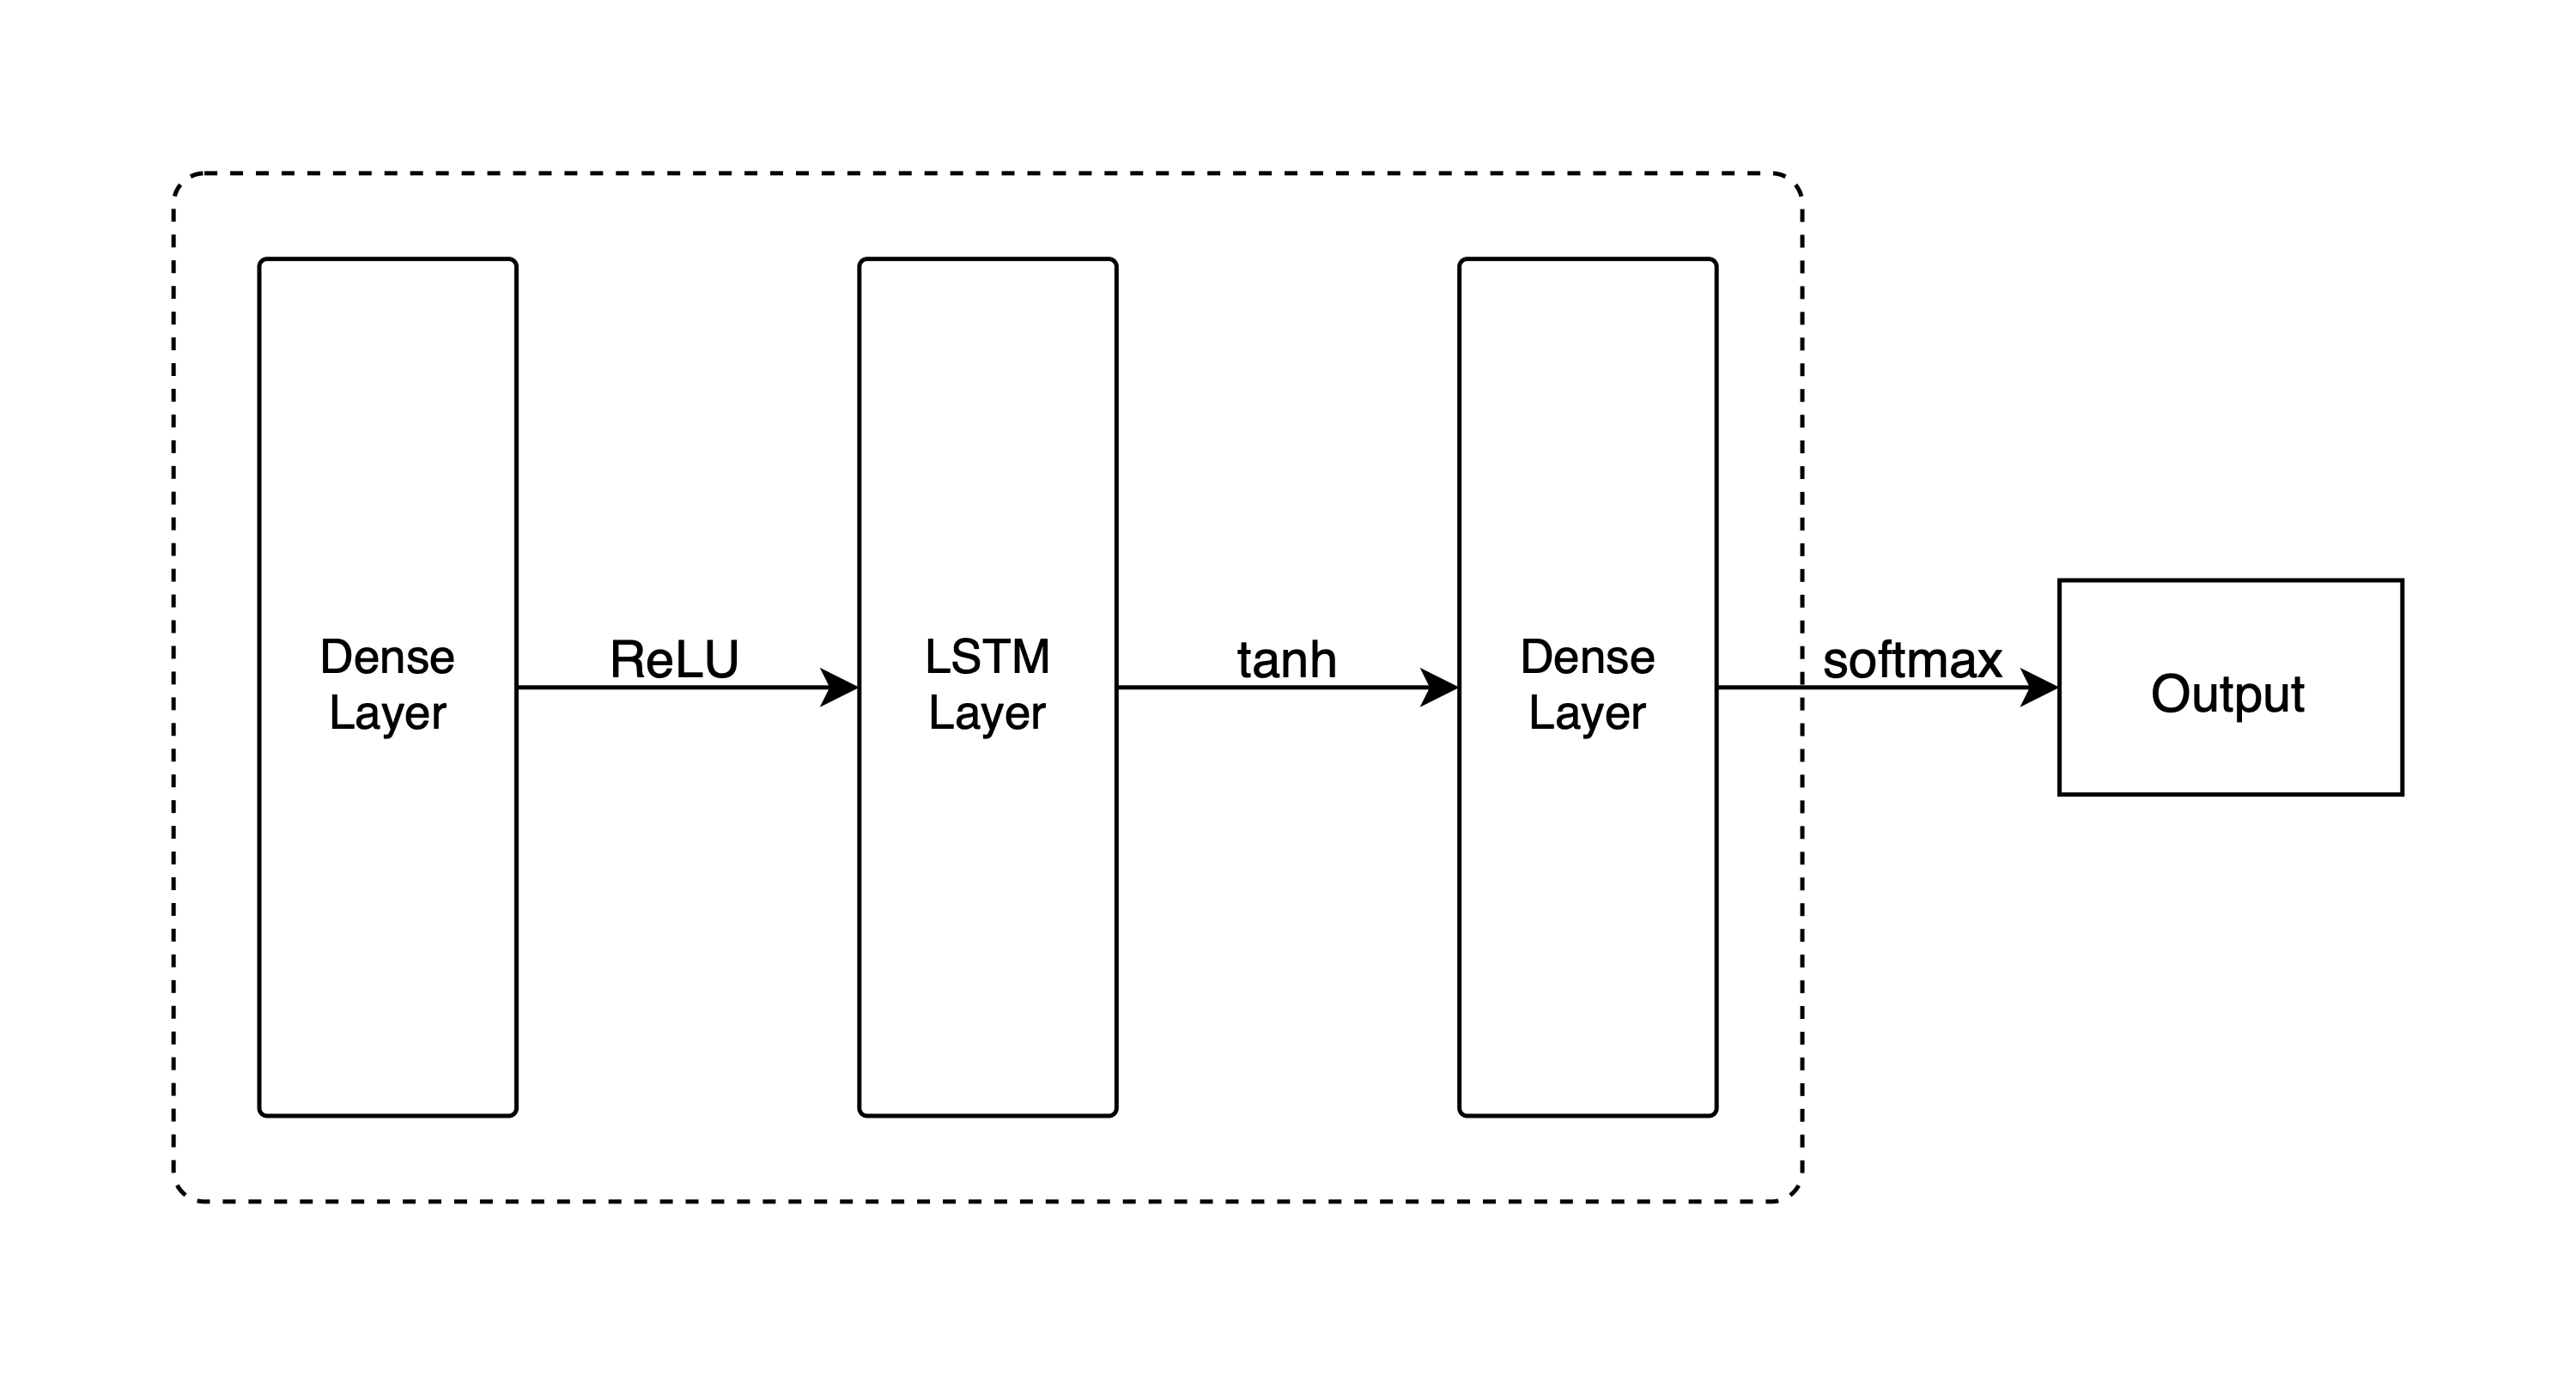
\includegraphics[width=1\textwidth]{media/overall_layers_with_funs.jpg}
        \caption{The architecture of both subsystems}
        \label{fig:system_architecture}
        \end{figure}
        

        The exact model architecture of the system is depicted in figure \ref{fig:system_architecture}. As in figures \ref{fig:ha_architecture} and \ref{fig:aa_architecture}, the input time frame(window) is fed to the two sub-systems, which have the same layer structure, as follows:
        \begin{itemize}
            \item \textbf{DENSE} layer with ReLU activation function
            \item \textbf{LSTM} layer containing 64 cells, using hyperbolic tangent activation function
            \item \textbf{DENSE} layer with softmax activation function
        \end{itemize}
        

        The input frame, first undergoes a linear transformation through the bottom Dense layer, then it is encoded into a latent space through the LSTM layer and finally through the top Dense layer a linear transformation is applied, to a space of the dimensionality of the respective target classes. Here, the softmax activation function as described in subsection \ref{subsec:activation_funs}, results in probabilistic outputs. The final prediction of each of the two subsystems would be the class with the highest probability.

        \subsection{Human Agent (HA)}
        The human agent predicts the human solo of the following step ($h\textsubscript{t+1}$ ) at each time-step $t$, as mentioned above. For this task, the HA's input data windows during the iterative process of successive predictions, include the expected human solo part that this sub-system learns to predict and the metric and lead sheet information channels which are one eighth ahead of the human solo. The accompaniment chords feature is excluded from the HA input. The output of this system, is single-step human solo information (the expected intentions of the soloist) -- one of the 128 possible piano-roll midi numbers, which will then be fed to the AA system as part of the input data window at each iteration.

        \begin{figure}[h]
        \centering
        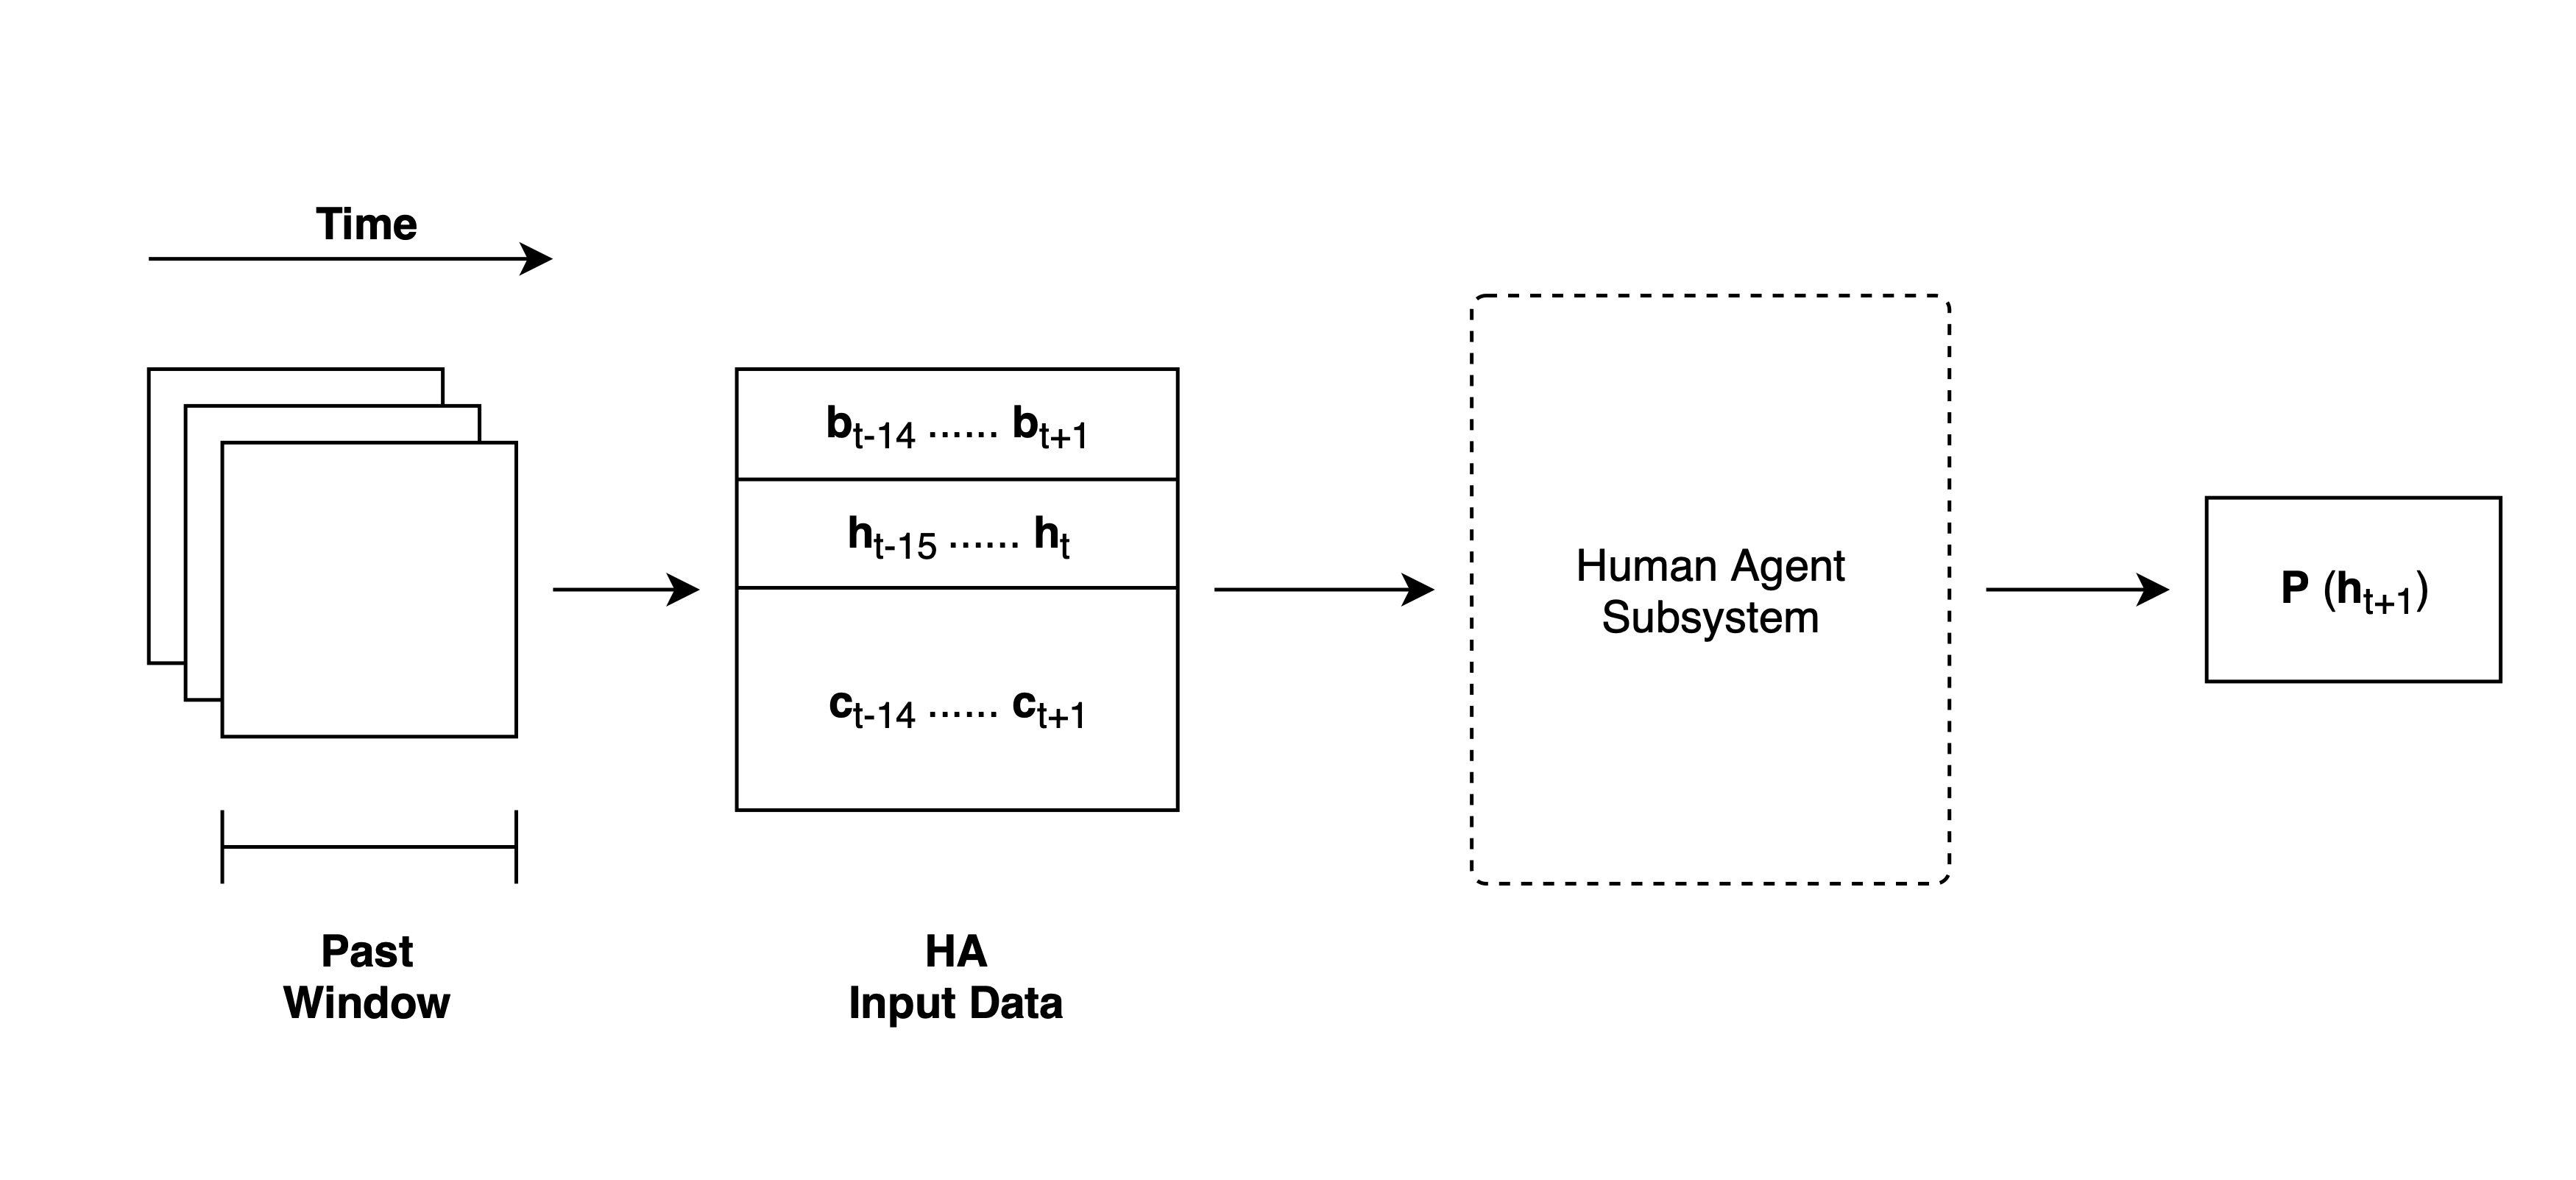
\includegraphics[width=0.8\textwidth]{media/ha_overall.jpg}
        \caption{The Human Agent Subsystem}
        \label{fig:ha_architecture}
        \end{figure}
        
        \subsection{Artificial Agent (AA)}
        The artificial agent, accordingly, predicts the accompaniment chord of step $t+1$ at each step $t$. This sub-system is dependent of all the data information channels, in contrast with the HA, therefore the input data windows during the prediction process, contain all the features mentioned in subsection \ref{subsec:overall_structure}. The AA's output is one of the dictionary's total accompaniment chord classes (dictionary construction details in subsection \ref{subsec:dict_info}).

        \begin{figure}[h]
        \centering
        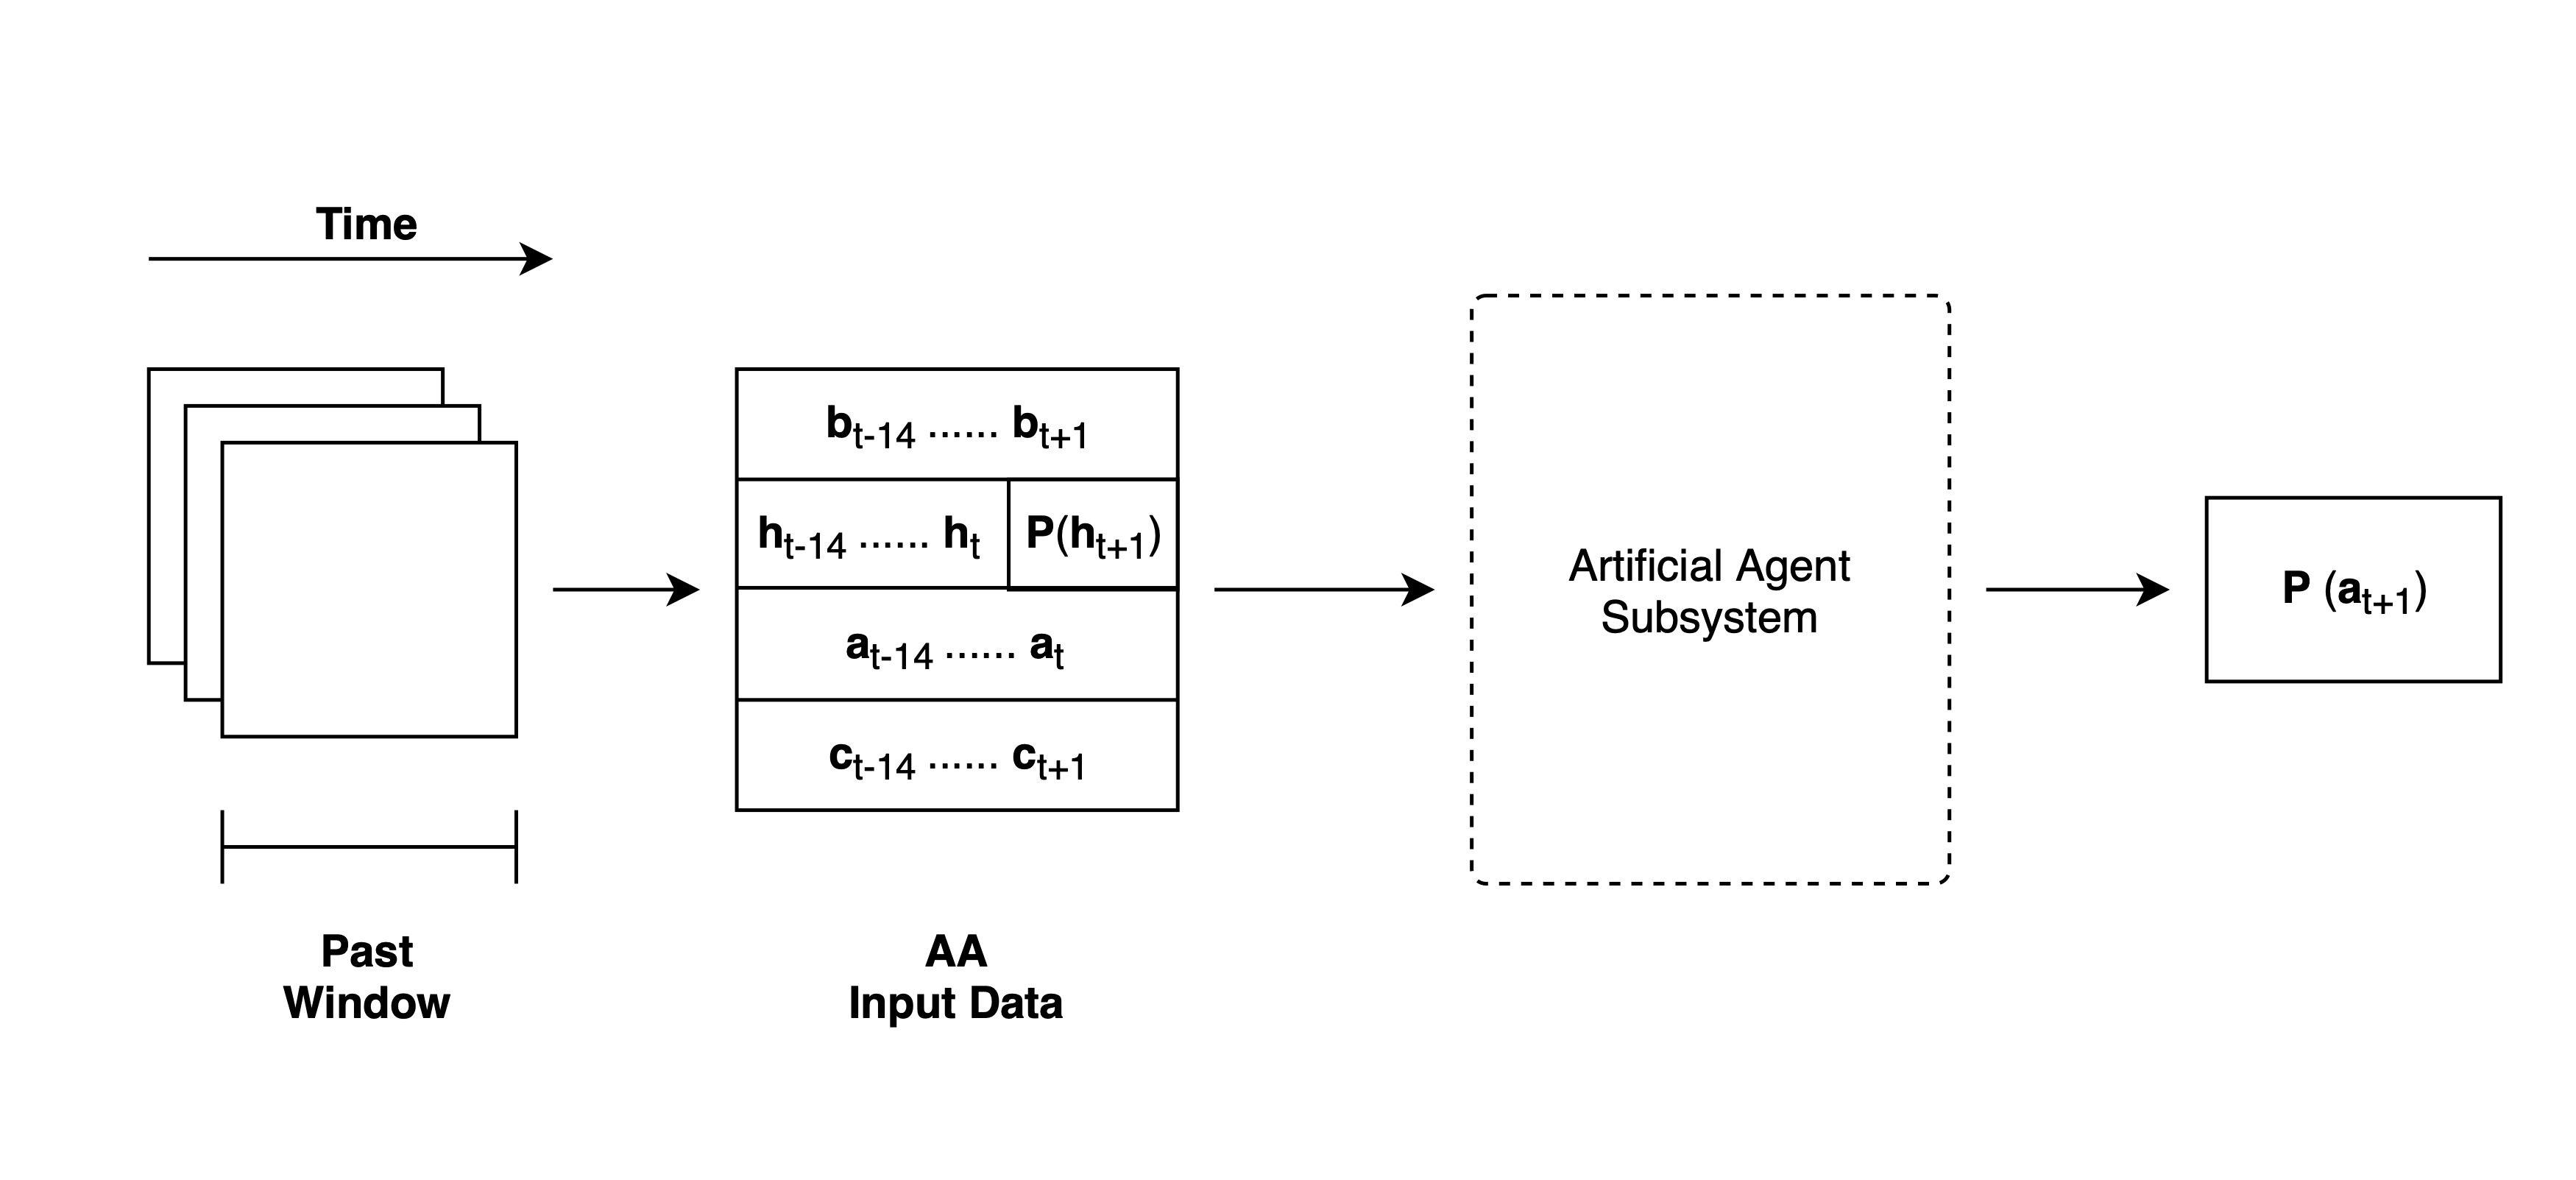
\includegraphics[width=0.8\textwidth]{media/aa_overall.jpg}
        \caption{The Artificial Agent Subsystem}
        \label{fig:aa_architecture}
        \end{figure}


        \subsection{Training}
        The system was trained for approximately 1200 epochs, with a batch size of 128 samples.  For the minimization of the categorical cross-entropy cost function, the Adam\textsuperscript{\cite{adam2014}} optimisation algorithm was used, with the learning rate set to 0.001 . The average time of the overall system's prediction was around 0.66 ms, 0.31 ms for the HA to predict the human solo and 0.35 ms for the AA to make the final prediction of the accompaniment chord. The loss of the training objective function in the validation set across the total epochs for which the models were trained, is shown in figure \ref{fig:val_loss}. 

        \begin{figure}[h]
        \centering
        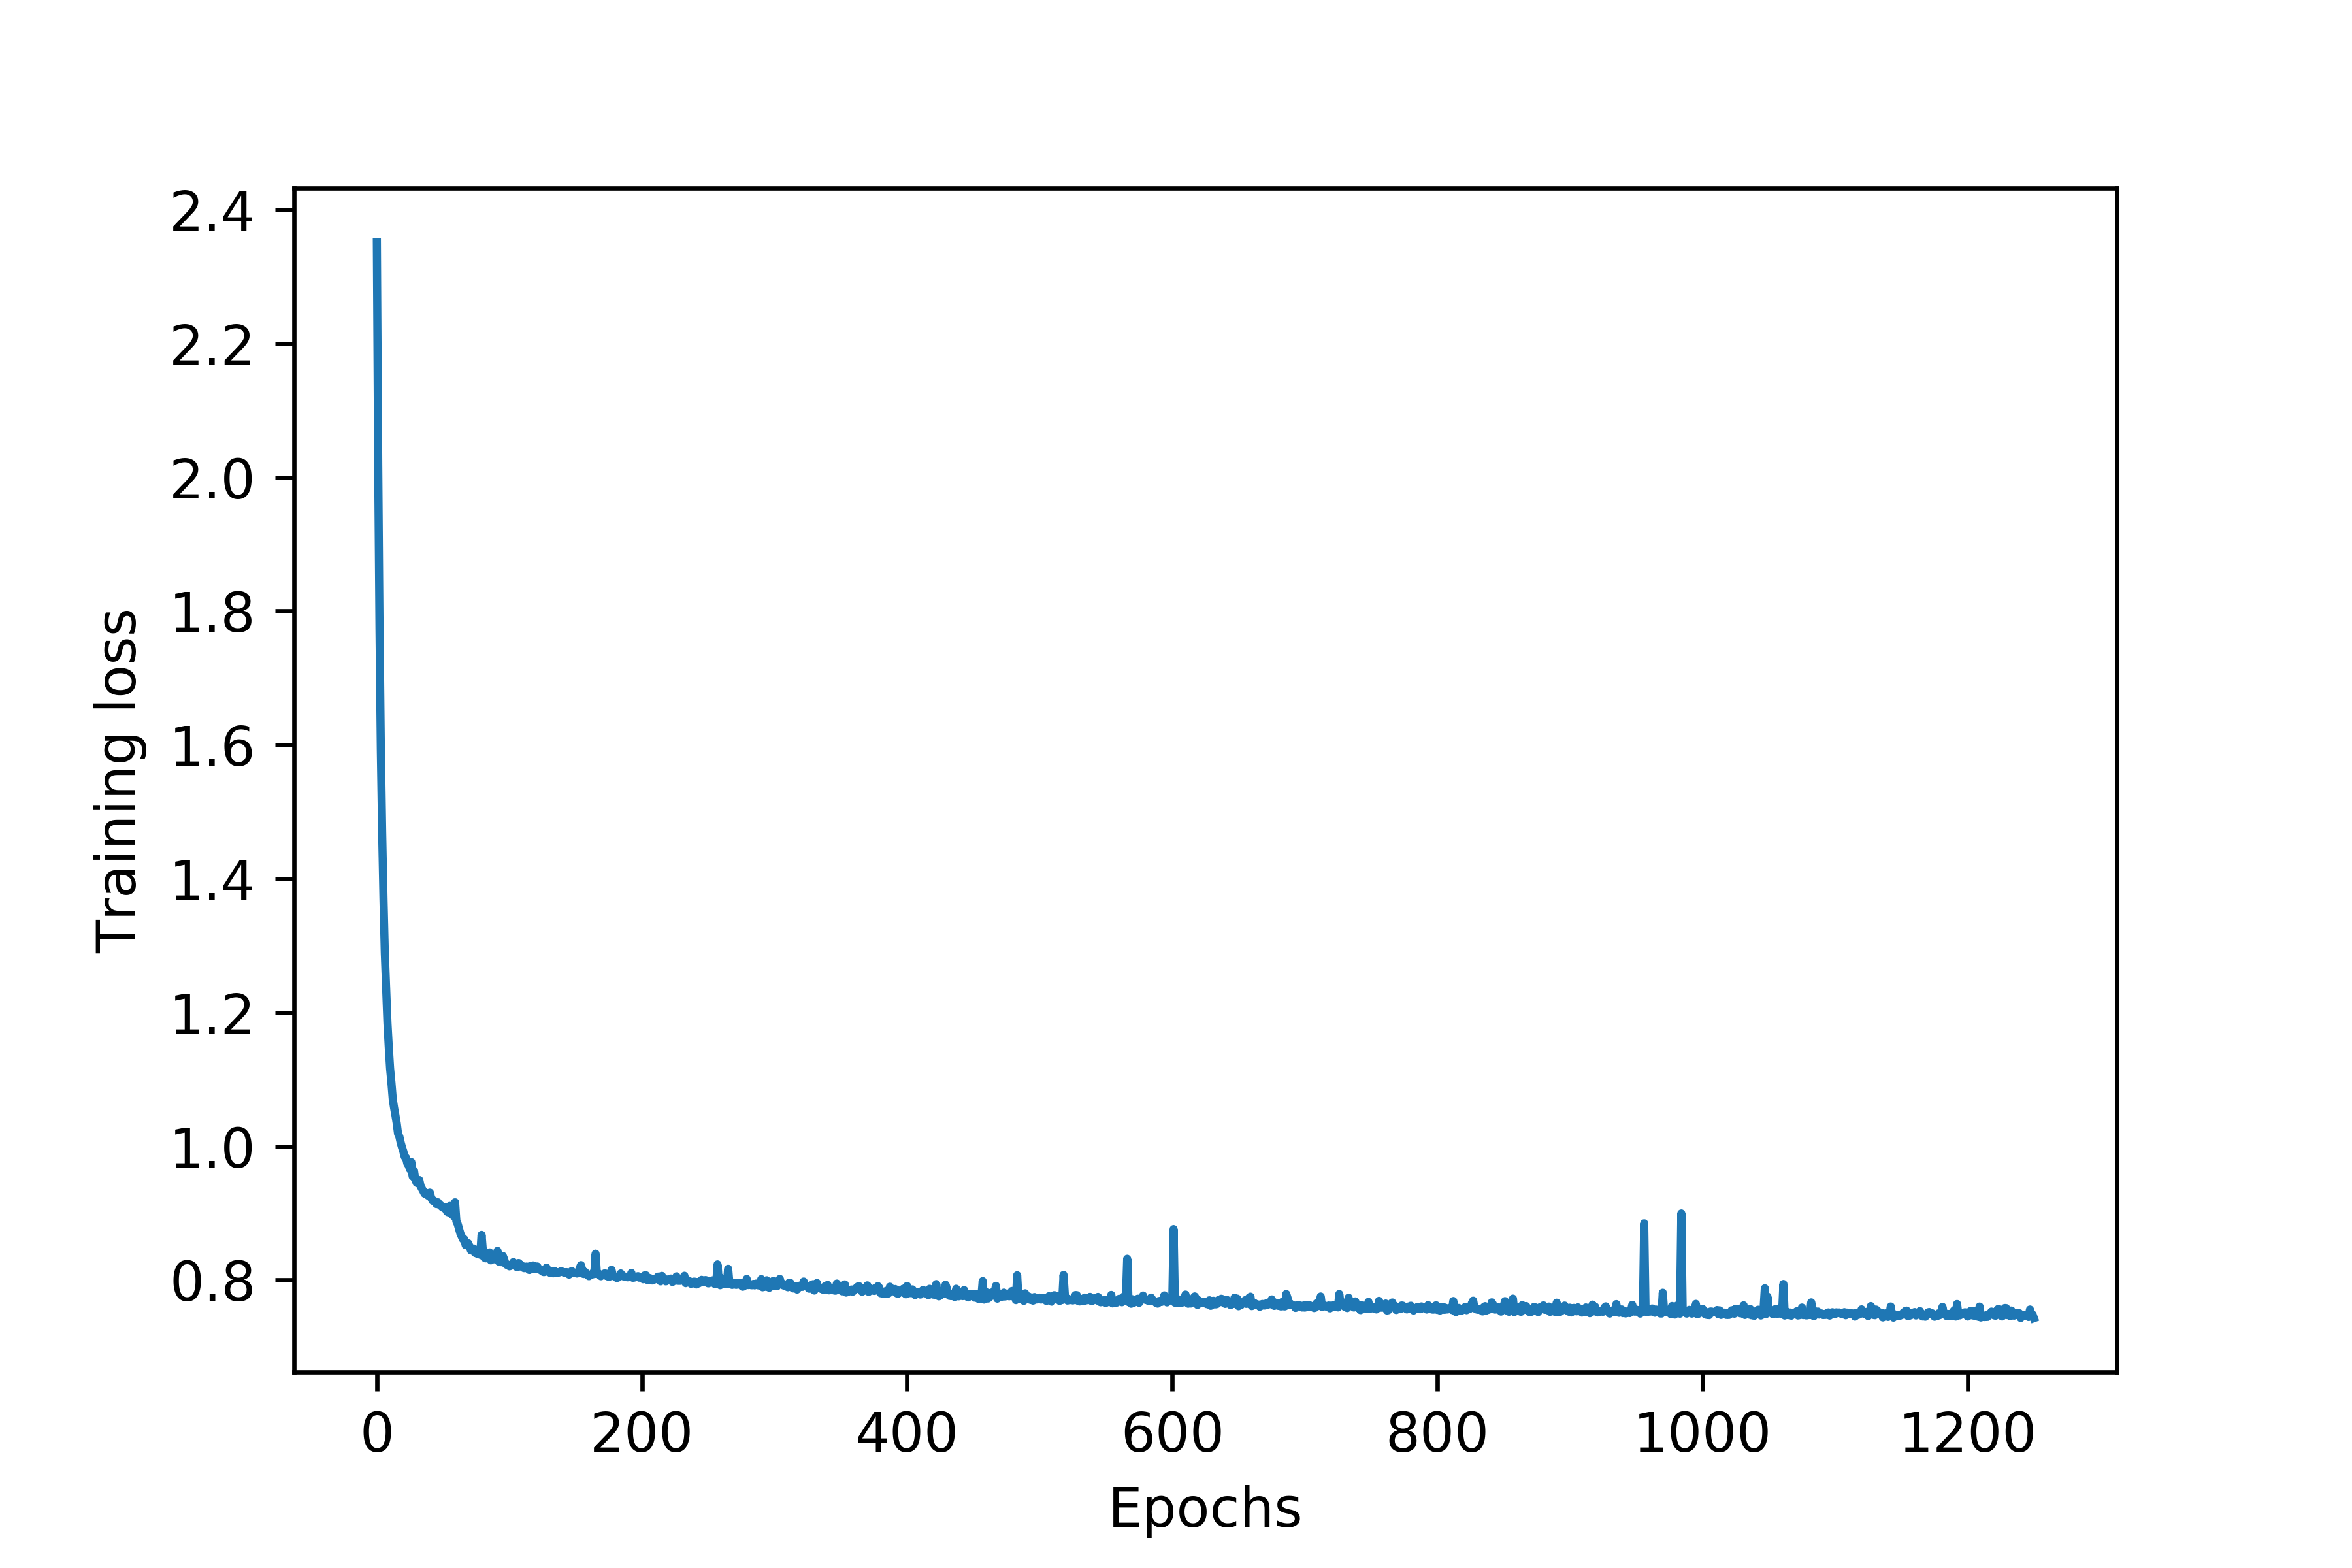
\includegraphics[width=0.65\textwidth]{media/epoch_val_loss_labels.png}
        \caption{Validation loss of the objective function over the total number of epochs of training}
        \label{fig:val_loss}
        \end{figure}

        \subsection{Real - Time Performance}
        A web application prototype has also been developed, based on MIDI.js and Tensorflow.js javascript libraries, aiming to test the degree in which the system is able to adapt to the solo input in a real time setting. 
    
        First, before the real-time performance, a number of measures to work on is defined as well as the metric structure and then the measures are filled with lead sheet chord information. The iterations are appointed by the metric structure, namely the duration of the measures (the amount of eighths they consist of). The interface developed for this task, saves the information added by the soloist, to feed the system after transforming it to a proper input representation.
        
        Each iteration deploys HA to predict human solo information of time-step $t+1$  ($P(h\textsubscript{t+1})$), being fed information about the past 16 time-steps ($[\ b\textsubscript{t-14}...b\textsubscript{t+1}\ ]$, $[\ h\textsubscript{t-15}...h\textsubscript{t}\ ]$, $[\ c\textsubscript{t-14}...c\textsubscript{t+1}\ ]$). The predicted output $P(h\textsubscript{t+1})$ is added to the data window of the AA, which will produce the accompaniment chord of time-step $t+1$ ($P(a\textsubscript{t+1})$), taking under account all the data features during the past 16 steps ($[\ b\textsubscript{t-14}...b\textsubscript{t+1}\ ]$, $[\ h\textsubscript{t-14}...h\textsubscript{t}\ P(h\textsubscript{t+1})\ ]$, $[\ a\textsubscript{t-15}...a\textsubscript{t}\ ]$, $[\ c\textsubscript{t-14}...c\textsubscript{t+1}\ ]$). After the produced accompaniment is played along with the soloist's input ($h\textsubscript{t+1}$), the predicted output $P(a\textsubscript{t+1})$ and the real-time inserted human solo information $h\textsubscript{t+1}$ are saved to the data used as the system's input, to keep them as the accompanying and human solo information of that specific future time-step $t+1$, respectively. 

    

\chapter{RESULTS} \label{chapter:results}
The results basically provide answers to the following research questions, raised in section \ref{sec:researchQuestions} :
    \begin{enumerate}
        \item To what extent the system is able to capture the harmonic lead sheet constraints.
        \item The impact of the different soloing styles on the proposed system.
        \item The suitability of the system to apply the proposed approach in real time settings.
    \end{enumerate}

For this purpose, two test jazz standards were examined (``All of me" and ``Au Privave") in different settings, simulating two extreme cases: 
    \begin{itemize}
        \item No notes: In this case, the human solo channel consists of consecutive rest occurrences. 
        \item Random notes: Here, randomly chosen notes within a range of two octaves, comprise the solo channel.
    \end{itemize} of no notes (case 1) and random notes (case 2) in the human solo channel. In this chapter, the system's responses in those scenarios are analyzed and examined, acquiring knowledge and feedback about the approach proposed. Sound samples of the system's output are publicly available on Github\footnote{\url{https://github.com/theatina/iJazzARTIST}}.
    
    \section{Jazz Standards} \label{sec:jazzStandards}
    Jazz standards are musical compositions that play an important role in jazz musicians' musical repertoire. A ``jazz standard” is held in continuing esteem and is commonly used as the basis of jazz arrangements and improvisations. 
    
    Not all jazz standards were written by jazz composers. Many are originally Tin Pan Alley popular songs, Broadway show tunes or songs from Hollywood musicals – the Great American Songbook. In Europe, jazz standards and "fake books" may even include some traditional folk songs (such as in Scandinavia) or pieces of ethnic music (such as gypsy melodies) that have been played with a jazz feel by well known jazz players. A commonly played song can only be considered a jazz standard if it is widely played among jazz musicians. The jazz standard repertoire has some overlap with blues and pop standards.
    
    The two jazz standards chosen to test the approach presented are the following : 
    \begin{itemize}
        \item All of Me ( popular song and jazz standard written by Gerald Marks and Seymour Simons in 1931 )
        \item Au Privave ( bebop jazz standard composed by Charlie Parker in 1951 )
    \end{itemize}    
    
    For the procedure, all the measures of each jazz standard were repeated four times in a row (forming the four quarters that are analyzed below), resulting in 40 measures in total. This construction allows us to perform thorough examination of the system's response by comparing and analyzing the respective generated chords.


    
    \section{Compliance with Lead Sheet Chords}
    A lead sheet is a musical composition comprising a chord progression and a melody line. A chord is a group of notes played simultaneously producing a distinct sound as a group. Because of their compactness, lead sheets provide a common means of representing music for both professionals and amateurs, often in the form of large collections known as ``fake books” \cite{keller2010impro}. The lead sheet does not explicitly describe the chord voicings, voice leading, bass line or other aspects of the accompaniment. Instead, these are specified later by an arranger or improvised by the performers \cite{benward1997music}. A lead sheet is often used by jazz musicians; one or more performers will play the melody line, while the rest of the ensemble improvises an accompaniment based on the chord progression given in the chord symbols, followed by an improvised solo also based on the chord progression.

    In this section, the ability of the system to capture the harmonic guidelines of the lead sheet is studied, which is the answer to the first question, stated in \hyperref[sec:researchQuestions]{Research Questions} above. The examination is conducted at pitch class set (PC-set) (set of all pitches with the same note name or its enharmonic equivalent) level, 
    that is, the chart chords and the system's interpretations, are indicated by their pitch class representation.  
    
    To examine the impact of the training on the system's harmonic compliance, data from different epochs (59 and 1251) were collected and presented below. 
    
    %------TABLES------%
    \input{chapters/tables/5_1.txt}
    \input{chapters/tables/5_2.txt}
    \input{chapters/tables/5_3.txt}
    \input{chapters/tables/5_4.txt}
    %------TABLES------%
        
    
    In tables \ref{tab:aom_chords_e59} and \ref{tab:aom_chords_e1251}, the chord symbols and the system's responses in the case of the ``All of me" jazz standard are shown, when no solo and random solo was provided. Similarly, tables \ref{tab:ap_chords_e59} and \ref{tab:ap_chords_e1251} present the respective results for the ``Au privave" jazz standard.

    The information on the system's performance and outcomes that can be drawn from the tables, lead to some conclusions. For example, regarding ``All of me", as presented in Tables \ref{tab:aom_chords_e59} and \ref{tab:aom_chords_e1251}, in most of the time-steps, the system was able to reflect the exact harmonic description in the lead sheet chart. The harmonic deviations which were mostly observed in the first few measures, are attributed to the system's delay in building memory for its decisions.
   

    \begin{figure}[!htb] 
    \centering
    \begin{tabular}{c}
        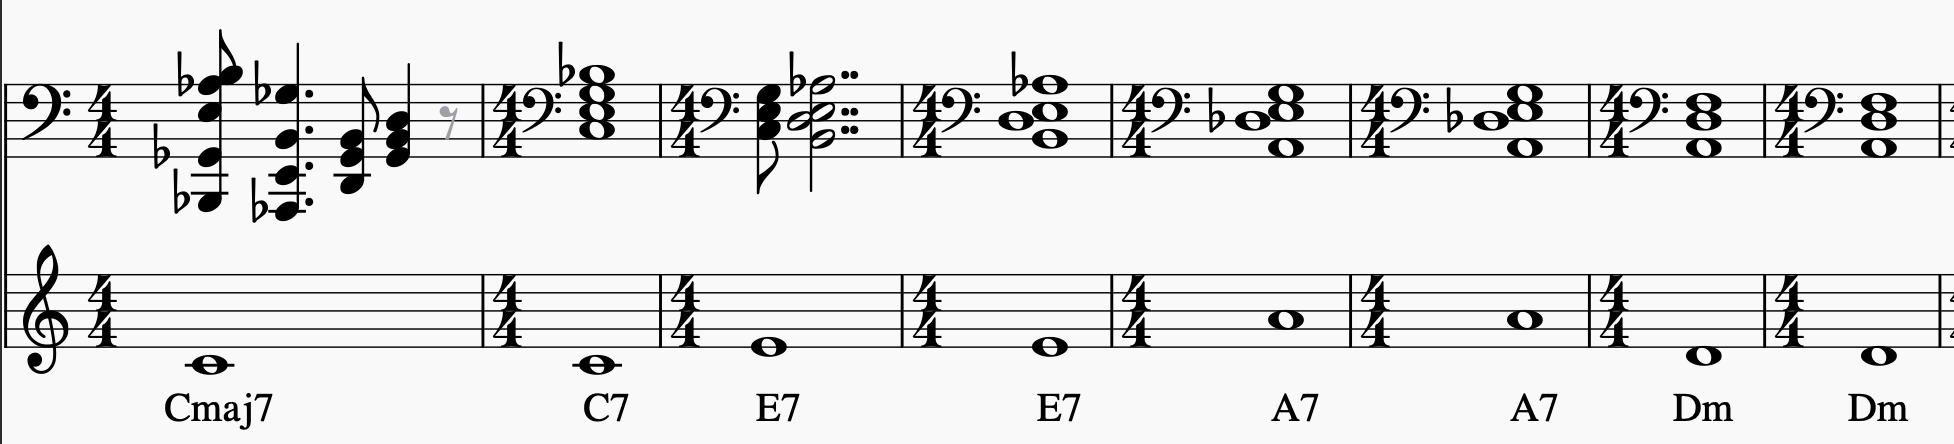
\includegraphics[width=0.9\textwidth]{media/aom_rand_bars1-8.png} \\
        (a) Bars 1-8 \\
        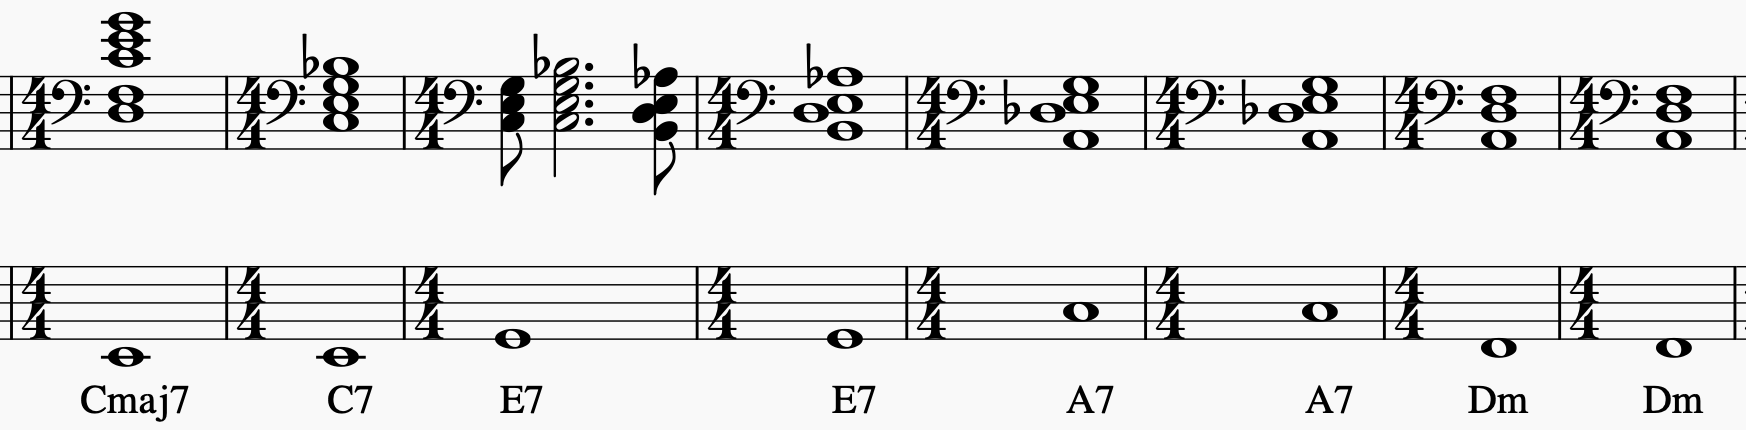
\includegraphics[width=0.85\textwidth]{media/aom_rand_bars33-40.png} \\
        (b) Bars 33-40
    \end{tabular}
    \caption{First 8 measures (a) and last 8 measures (b) of system-generated chords over the respective lead sheet chords for ``All of Me'' with random solo part.}
    \label{fig:aom_beginning_comparison}
    \end{figure}

    Figure \ref{fig:aom_beginning_comparison}, shows the first 8 (1-8) and final 8 (33-40) measures of the system's output chords, under the ``All of me" jazz standard lead sheet in real time. In this instance, the solo was a sequence of random notes, omitted from the system's output depiction in the figure. The first three chords of the first measure, indicate the aforementioned delay of the system to capture and comply with the given constraints, as they comprise inaccurate choices for the respective lead sheet chord. Additionally, in some cases, the system has shown inability to follow the unexpected chord changes, such as the transition from the Cmaj7 (C major seventh) chord ( [0,4,7,11] ) to the E7 (E seventh) chord ( [2,4,8,11] ), shown in measures 2-3 ( \ref{fig:aom_beginning_comparison}(a) ) and 34-35 ( \ref{fig:aom_beginning_comparison}(b) ) of the figure. 

    %Finally, compared to epoch 59 ( Table \ref{tab:aom_chords_e59} ), after the 1251st epoch of training, the lead sheet chords are   \ref{tab:aom_chords_e1251} shows better ...

    Similarly, the output chords of the system over the ``Au privave" jazz standard lead sheet chords are shown in Tables \ref{tab:ap_chords_e59} and \ref{tab:ap_chords_e1251}, following a resemblant compliance pattern but demonstrating fewer inaccurate interpretations.

    \section{Variability}
    
    The system's generated chords of each piece in each scenario, are expected to differ, as the human solo improvisations are considered to have an impact on the system's response, which is examined through direct comparison between the two pieces in each case.

    \input{chapters/tables/5_5.txt}
    \input{chapters/tables/5_6.txt}
    \input{chapters/tables/5_7.txt}
    \input{chapters/tables/5_8.txt}

    In order to study the variability of the system-generated chords, quartile similarities were computed and shown in Tables \ref{tab:aom_quartile_59} and \ref{tab:aom_quartile_1251} regarding the ``All of me" piece and Tables \ref{tab:ap_quartile_59} and \ref{tab:ap_quartile_1251} for the ``Au Privave" jazz standard. More explicitly, this similarity indicates the normalized percentage of different chords per time step during the accompaniment process, over four repetitions(``quartiles") of each chart, with random and without solo.  
    
    It was calculated that in ``All of Me”, the percentage of system-generated chords that are different between random and no solo for epoch 59 is only 2\%, which rises to 60\% after training the system for 1251 epochs, showing that the impact of the solo in the system's response is more remarkable in early epochs, compared to the effect of its presence as epochs progress. In ``Au Privave” the same percentage ranges from 74\% after epoch 59 and reaches 84\% at epoch 1251, leading to the conclusion that the presence of the solo has greater impact on the system's generations for this particular piece. The results of the comparison between each improvisation scenario which are depicted in the tables mentioned above, led to the conclusions extensively discussed below.

    In ``All of Me” under the setting of no solo, only the first repetition differs from the remaining three, in both epochs 59 and 1251 of the system's training, as shown in Tables \ref{tab:aom_quartile_59} and \ref{tab:aom_quartile_1251}, in their first rows and columns. However, as observed from the similarity in the case of random solo, the response in the early epoch was not affected in general, while in the late epoch the influence of the solo is shown to be strong. Overall, the artificial agent's variability in the presence of random solo, concerning ``All of me", indicates the system's responsiveness to the human agent's input, after being trained for multiple epochs (1251 in this case). In contrast, regarding ``Au Privave", the system has generated variations of the lead sheet chart for each iteration, even from the early epoch ( 59 ), as well as demonstrated more conspicuous variability after more epochs (1251). 

    Another means of comparison in the terms of the system's variability, is the total number of different voicings generated for each chord symbol of the chart, with variations of their layouts being note doublings or inversions to name a few. 

    \begin{figure}
    \centering
    \begin{tabular}{cc}
        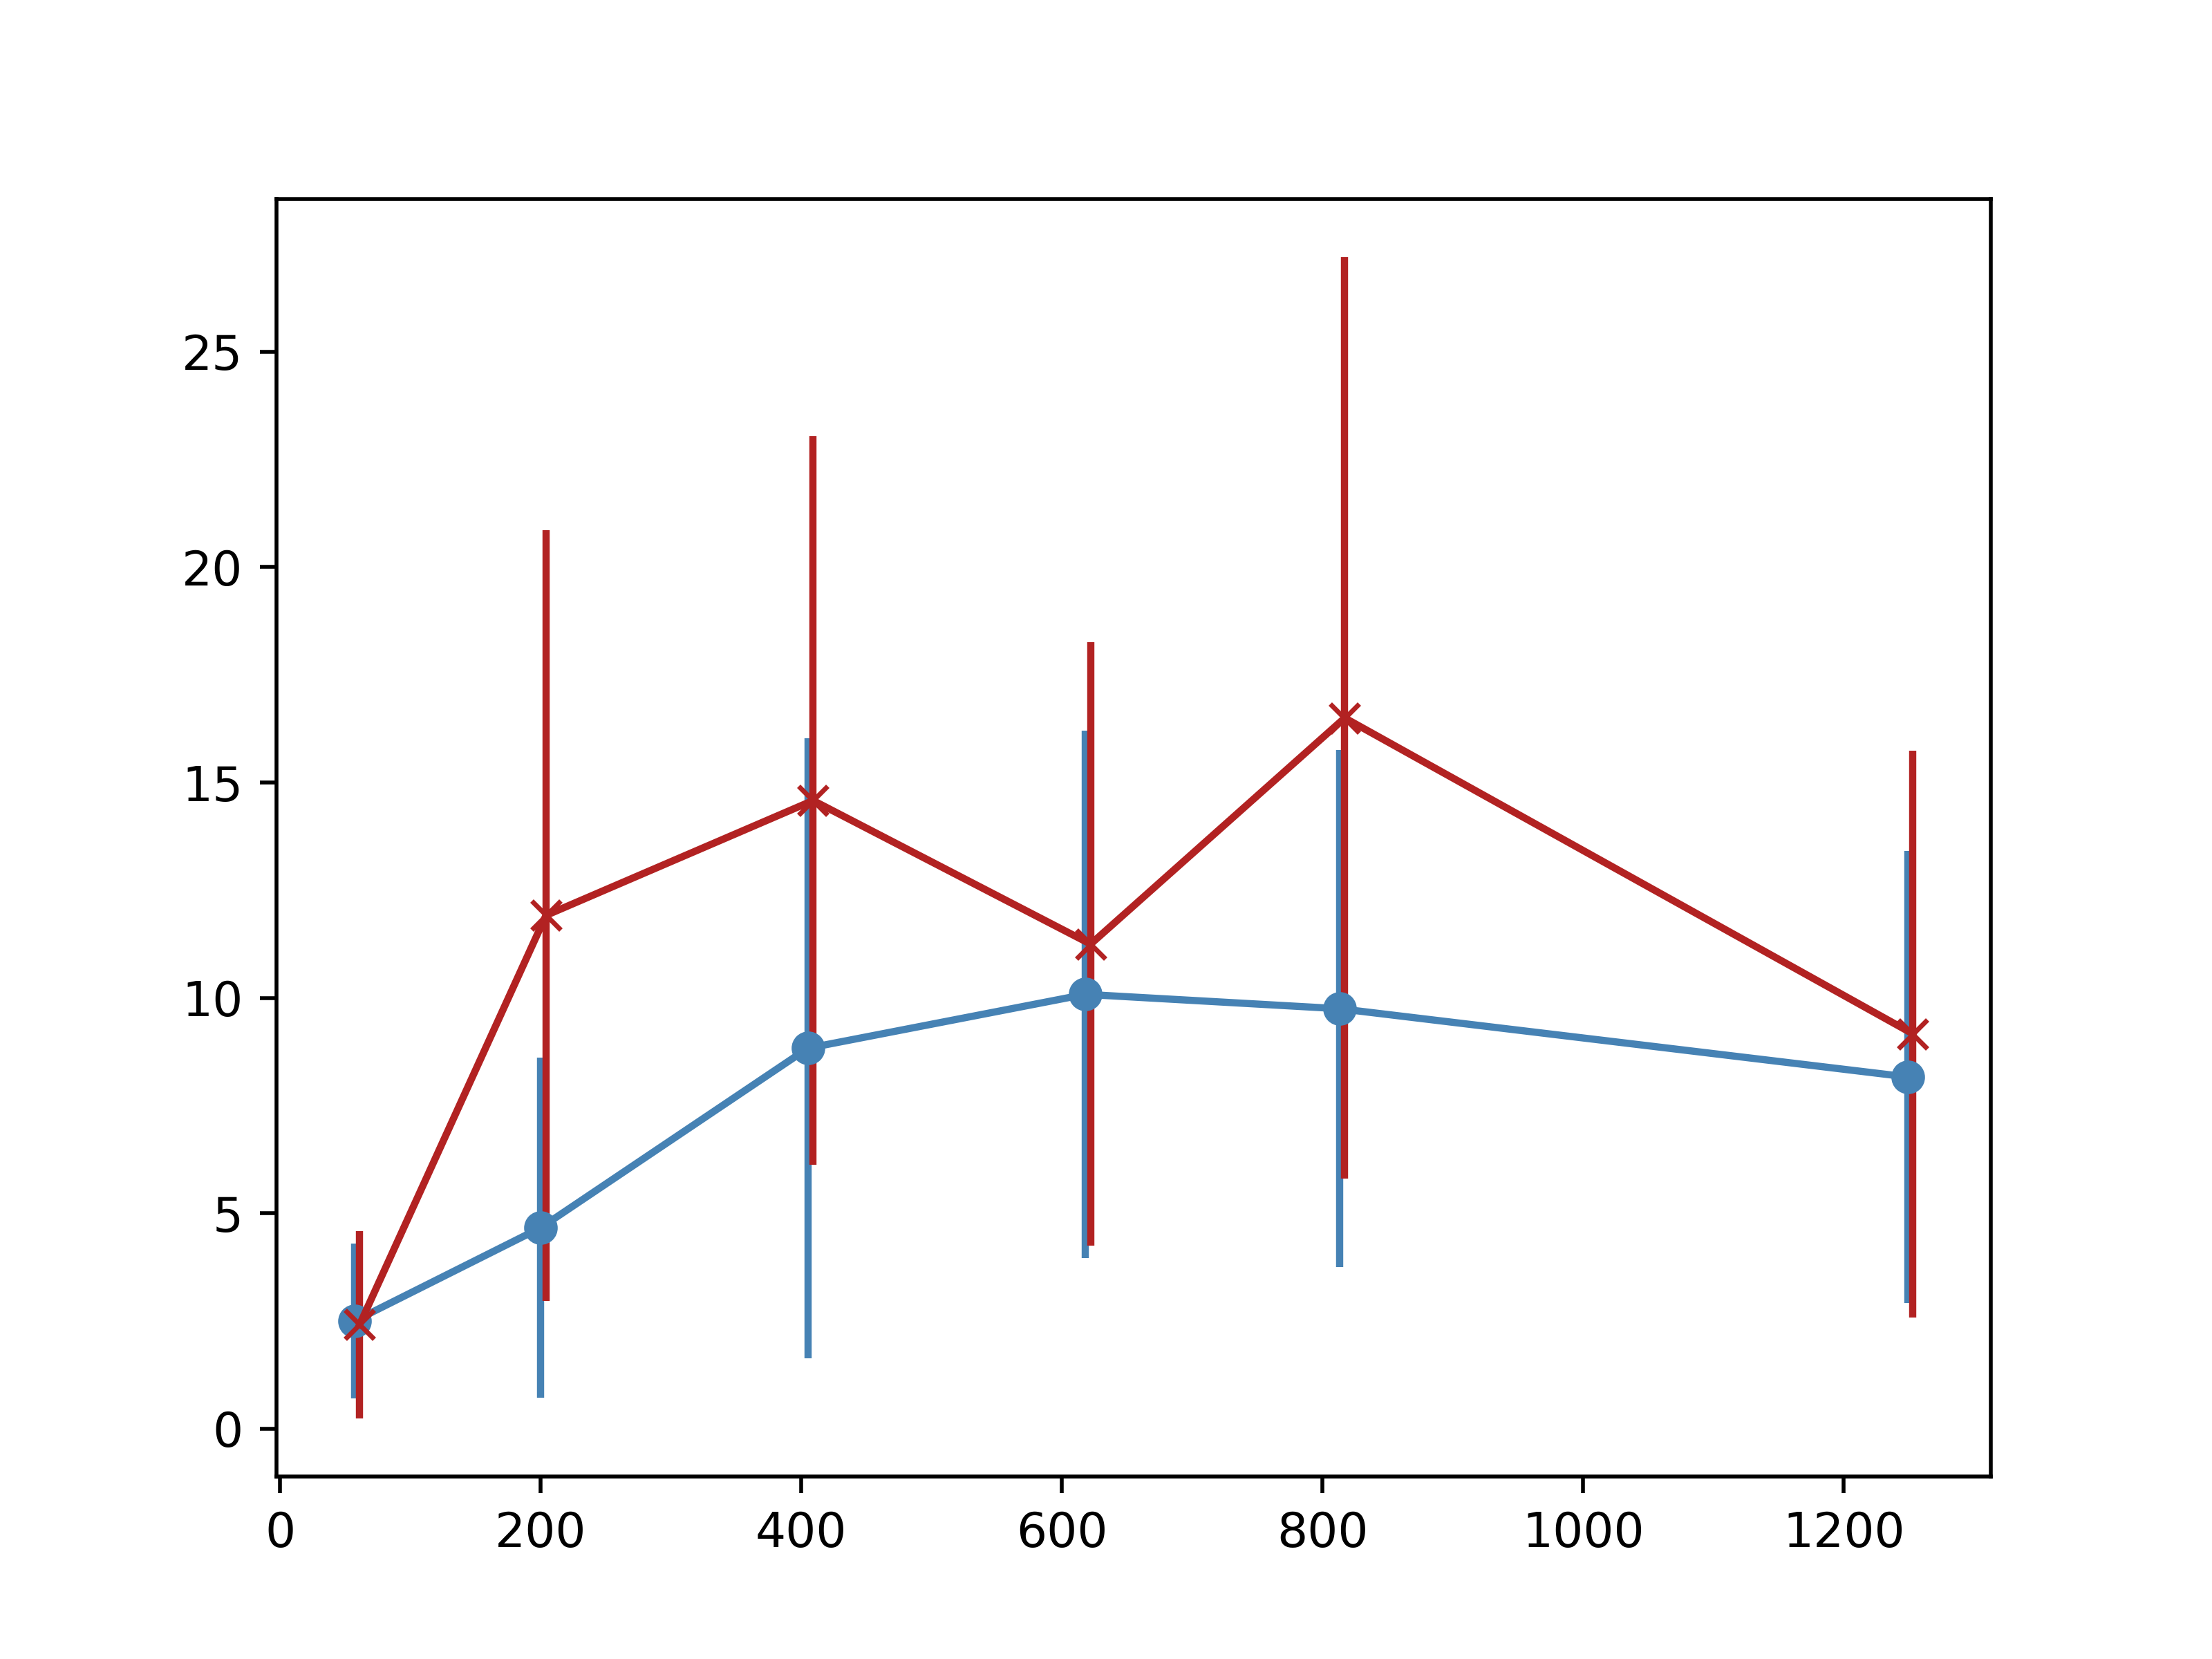
\includegraphics[width=0.5\textwidth]{media/aom_voicings_errorbars.png} & 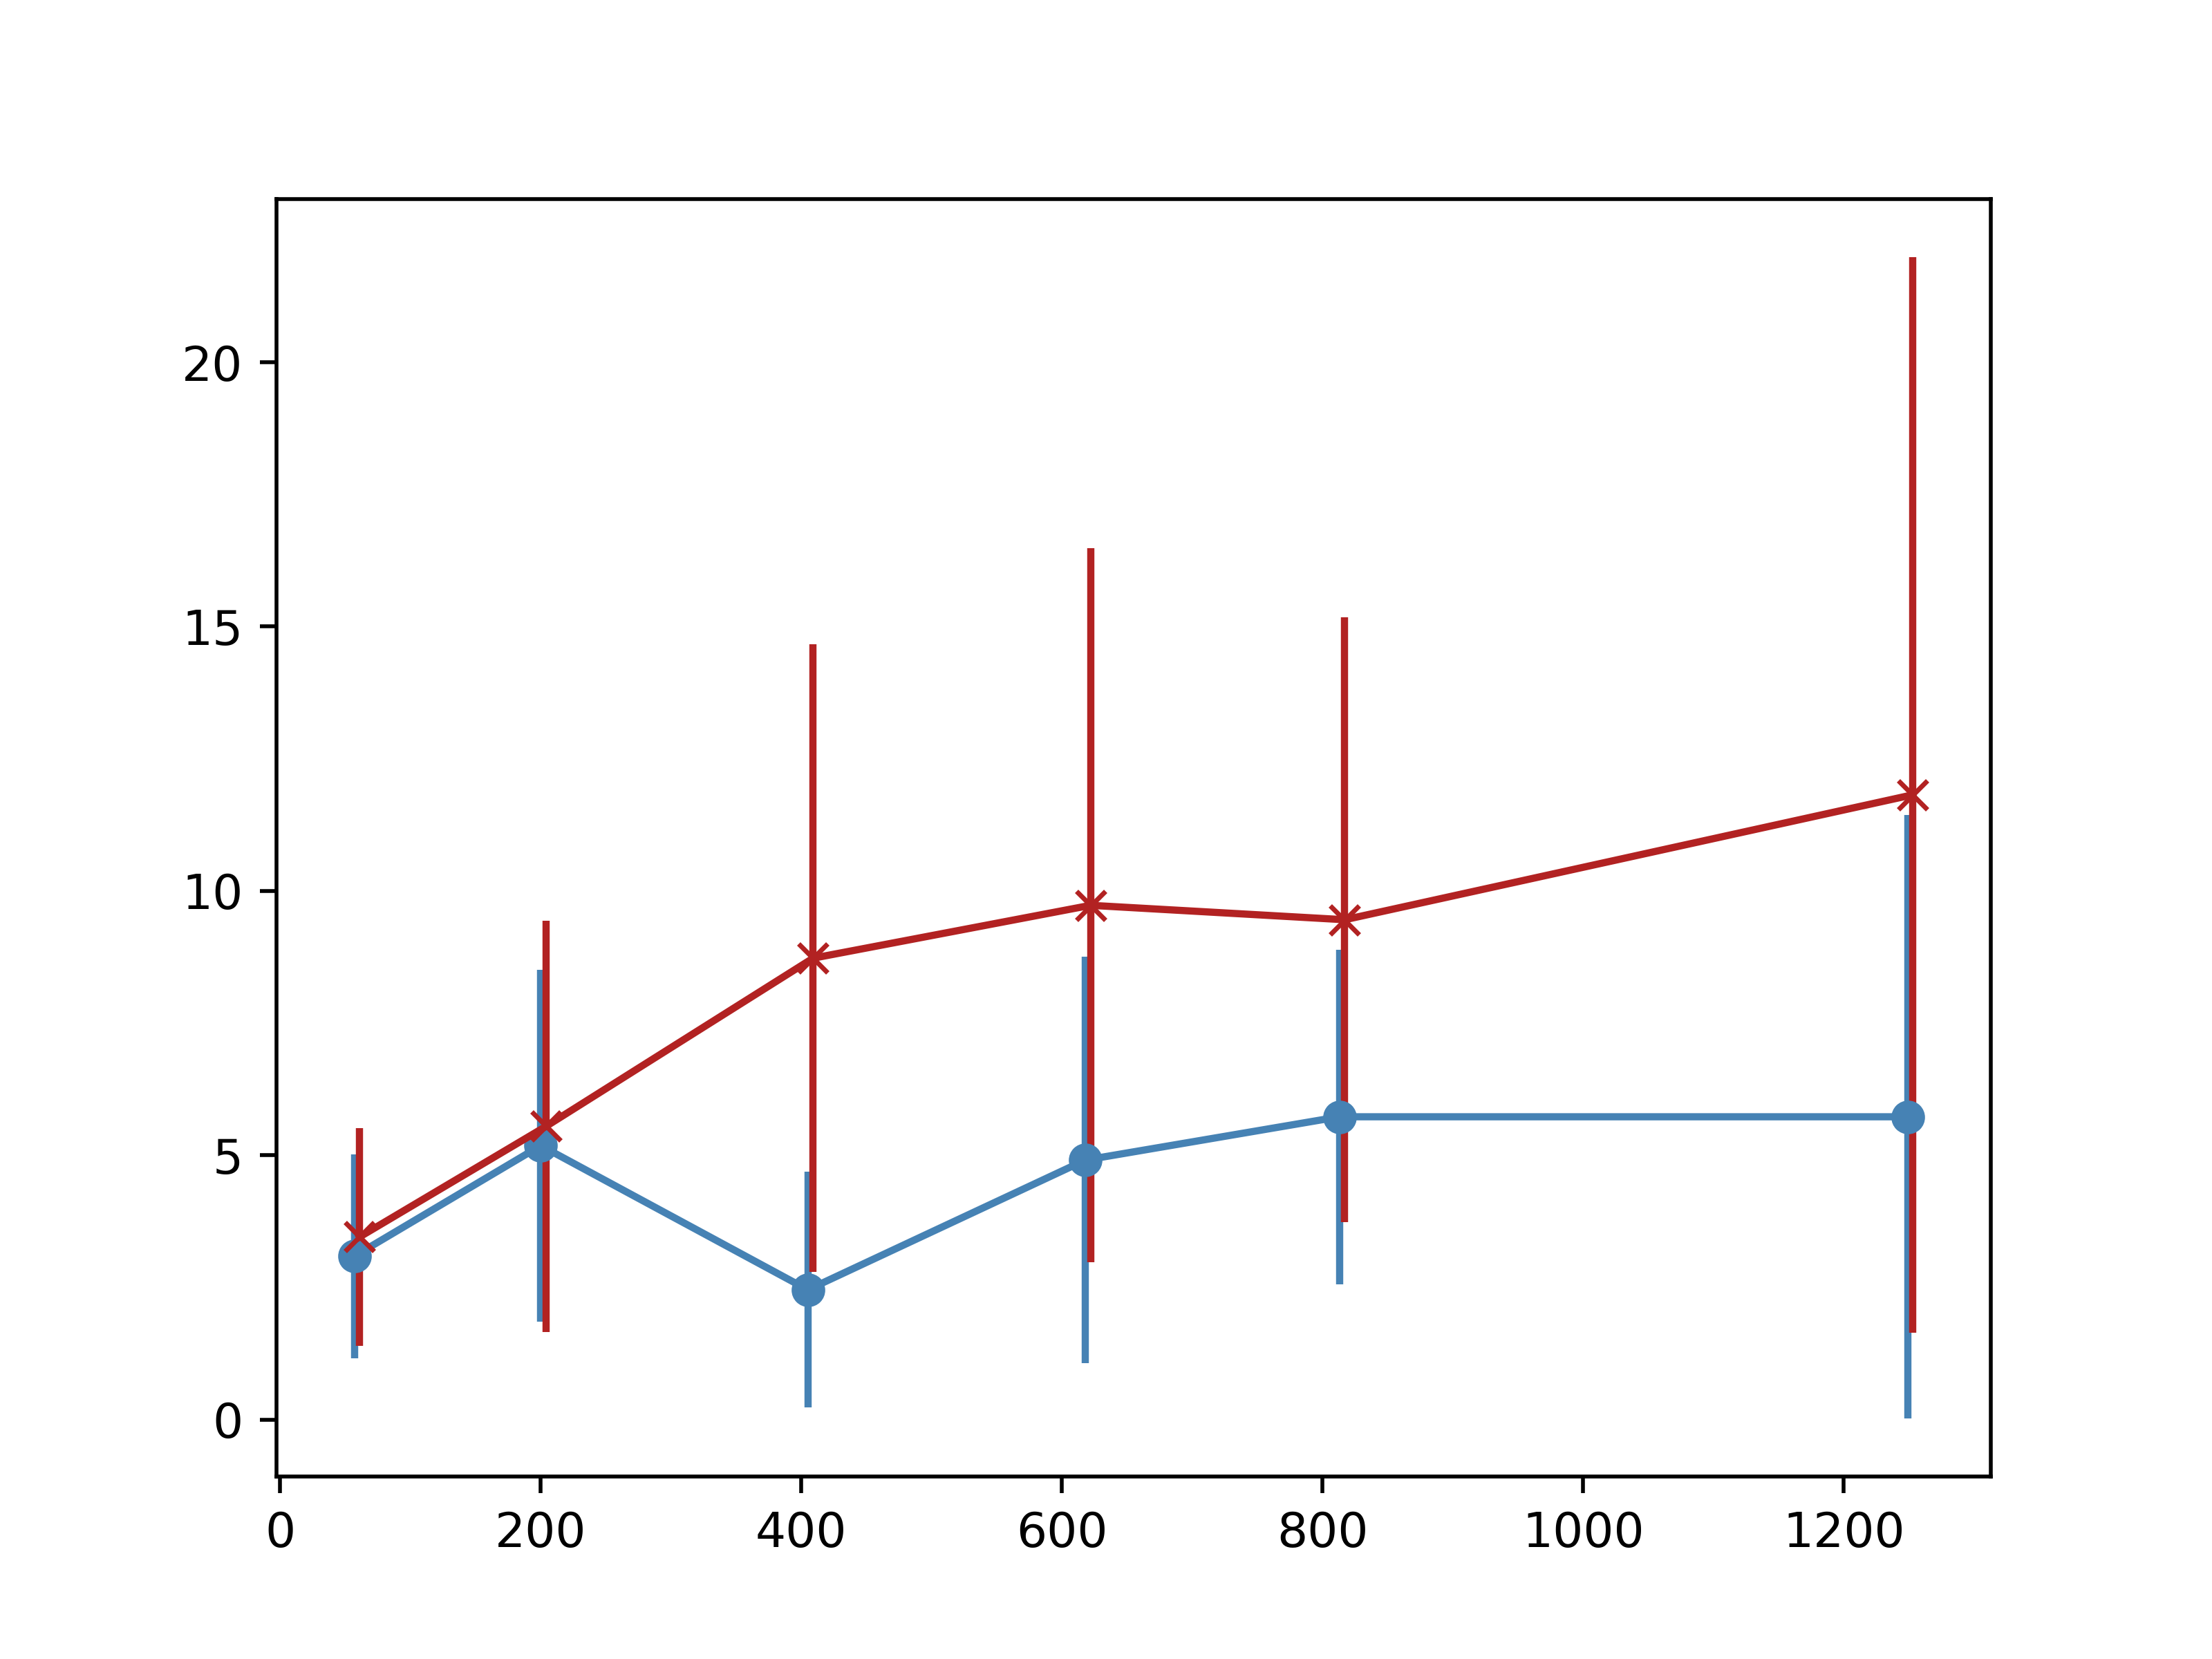
\includegraphics[width=0.5\textwidth]{media/ap_voicings_errorbars.png} \\
        All of me & Au Privave
    \end{tabular}{}
    \caption{Error-bars of different voicings generated for each chord label in the chart over a set of sampled epochs, in the presence of random solo (red) and absence thereof (blue).}
    \label{fig:voicings}
    \end{figure}{}

    In Figure \ref{fig:voicings}, the different voicings for each chord label of the chart are shown, over a set of randomly chosen epochs from the total epochs of the system's training. As indicated in the figure, in ``All of me", at the 59th epoch of the training, the system  generated approximately 2.5 variations of chord voicings and proved to be independent of the solo presence, which is not the case in later epochs, as the variability dependence on the solo increases as the epochs progress. Also, in ``Au Privave", the growing tendency of dependency on the solo is more evident, as the epochs increase. Finally, thorough concurrent examination of Figures \ref{fig:val_loss} and \ref{fig:voicings}, leads to the conclusion that there is a correlation between the objective function loss and the system's adaptability to the human solo, with lower loss values (further training) providing greater variability of the system. 
    
    % \clearpage
    % \section{Audio Samples}
    % \begin{center}

\includemedia[
  transparent,
  passcontext,
  addresource=./chapters/soundFiles/jack5.mp3,
  flashvars={source=./chapters/soundFiles/jack5.mp3},
]{\color{blue}\framebox[0.4\linewidth][c]{Audio sample}}{APlayer.swf}
% \caption{Audio sample from the generated accompaniment for the the `` " jazz standard with no solo.}
\end{center}

\chapter{CONCLUSIONS AND FUTURE WORK} \label{chapter:conclusions_futurework}
    \section{Conclusions}
    This work, has carried out research on the task of real-time jazz improvisation, a collaborative process between a human and artificial agent, based on predefined chord charts, through implicit machine learning techniques. The main purpose of the thesis was to study the employment of deep NNs for the aforementioned matter, the ability thereof to model the expectation and its violation in jazz improvisation scenarios and the artificial agent's ability to develop a model of expectation for the intentions of the human soloist. Additionally, data refinements have been applied to obtain greater variability of the accompaniment of the pieces in the dataset. 

    Testing of the system was performed within two simulated cases of real-time scenarios, accompaniment generation over a random and no solo. The resulting responses under the two jazz standard settings described in \hyperref[sec:jazzStandards]{\textbf{Jazz Standards}} section, have indicated the largely achieved compliance of the system with each chord chart, disregarding the first few time steps of the process, during which the system was considered to be building up memory. The aforementioned behaviour can possibly be attributed to the LSTMs' operational structure and their random initialisation states. Moreover, in the case of ``All of me", the system proved to be unaffected by the simulated human solo, as well as characterised by repetition, in most accompaniment sessions. In contrast, ``Au Privave" has demonstrated greater dependence on the randomly constructed solo, conclusion drawn from the demonstrated decrease in self-repetition and increase in the variability of voicings over particular chart chords.  

    \section{Future Work}
    %In order for the real-time accompaniment system to be studied more profoundly in terms of the proposed task, further research is imperative. 
    The results of the study indicate the capability of modeling the violation of expectation for jazz accompaniment in a real-time scenario by employing deep NNs. However, some limitations have emerged, concerning the dataset as well as the computational complexity. 

    The lack of proper datasets that incorporate all the information needed for the task (lead sheet chords, metric information, solo and accompaniment), raised the need for data construction or refinement and integration thereof to the initial dataset. For instance, data enrichment was performed, aiming to increase the dataset's variability, using rudimentary probabilistic methods, which in some cases renders the transitions inconsistent, difficult to be learnt from the system. 

    Regarding the music style, the most common genre found in the datasets available up to this point is pop, which is characterised by less variability compared to jazz music. Therefore, a dataset based on jazz standard accompaniment is of utmost importance for proper examination of the discussed hypothesis. 

    Within the scope of real-time application of the developed system, the execution time also has proven to be marginally acceptable for performing the task. In order to comply with the real-time setting to a degree, the time resolution that was applied to the dataset, has constrained the system in terms of expressive capabilities both for capturing the human agent's characteristics and for creating the accompaniment for the solo.

     
\backmatter

% abbreviations table
\abbreviations
% \begin{center}
% 	\renewcommand{\arraystretch}{1.5}
% 	\begin{longtable}{ l @{\qquad} l }
% 	\toprule
%         AA & Artificial Agent \\
\hline
AI & Artificial Intelligence \\
\hline
ANN & Artificial Neural Network \\
\hline
BN & Bayesian Network \\
\hline
CA & Cellular Automata \\
\hline
CNN & Convolutional Neural Network \\
\hline
DSP & Digital Signal Processing \\
\hline
FL-Systems & Finite L-Systems \\
\hline
GAN & Generative Adversarial Network \\
\hline
GRU & Gated Recurrent Units \\
\hline
HA & Human Agent \\
\hline
HMM & Hidden Markov Model \\
\hline
LSTM & Long Short-Term Memory \\
\hline
L-Systems & Lindenmayer Systems \\      
\hline
NN & Neural Network \\
\hline
ReLU & Rectified Linear Unit \\
\hline
RNN & Recurrent Neural Network \\
\hline
SI & Swarm Intelligence \\ 
\hline
SVM & Support Vector Machine \\
% 	\bottomrule
% 	\end{longtable}
% \end{center}

\begin{center}
\renewcommand{\arraystretch}{1.5}
\begin{tabularx}{0.8\textwidth} { 
  | >{\raggedright\arraybackslash}X 
  | >{\raggedright\arraybackslash}X 
  | }
 \hline
 AA & Artificial Agent \\
\hline
AI & Artificial Intelligence \\
\hline
ANN & Artificial Neural Network \\
\hline
BN & Bayesian Network \\
\hline
CA & Cellular Automata \\
\hline
CNN & Convolutional Neural Network \\
\hline
DSP & Digital Signal Processing \\
\hline
FL-Systems & Finite L-Systems \\
\hline
GAN & Generative Adversarial Network \\
\hline
GRU & Gated Recurrent Units \\
\hline
HA & Human Agent \\
\hline
HMM & Hidden Markov Model \\
\hline
LSTM & Long Short-Term Memory \\
\hline
L-Systems & Lindenmayer Systems \\      
\hline
NN & Neural Network \\
\hline
ReLU & Rectified Linear Unit \\
\hline
RNN & Recurrent Neural Network \\
\hline
SI & Swarm Intelligence \\ 
\hline
SVM & Support Vector Machine \\
\hline
\end{tabularx}
\end{center}


% % appendix
% \begin{appendix}
% % mark the beginning of the appendix
% \appendixstartedtrue

% % add appendix line to ToC
% \phantomsection
% \addcontentsline{toc}{chapter}{APPENDICES}

% \chapter{FIRST APPENDIX}
% \chapter{SECOND APPENDIX}
% \chapter{THIRD APPENDIX}
% \end{appendix}

% manually include the bibliography
\bibliographystyle{refs_style}

% set font size (10pt) for bib entries
{\fontsize{10pt}{1}\selectfont
\bibliography{refs}}

% \bibliography{refs}
% \printbibliography
% include it also in ToC (do sth on your own)
\addcontentsline{toc}{chapter}{REFERENCES}


\end{document}
